% !TeX program = xelatex
\documentclass[a4paper,10pt]{article}

% ============================================================================
% កញ្ចប់សម្ភារៈសិក្សាបោះពុម្ព ស-ខ្មៅ (Printable Classroom Materials - Grade 8 HL & Incenter)
% ត្រូវគ្នា ១០០% នឹង LS_Plan_HL.tex និង Teaching_Scenario_HL.tex
% ============================================================================
\usepackage[a4paper, left=1.0cm, right=1.0cm, top=0.75cm, bottom=1.05cm, footskip=0.55cm]{geometry}
\usepackage{amsmath, amssymb}
\usepackage{unicode-math}
\usepackage{fontspec}
\usepackage{array, colortbl}
\usepackage[table]{xcolor}
\usepackage{enumitem}
\usepackage{pifont}
\usepackage{fancyhdr}
\usepackage{lastpage}
\usepackage{tikz}
\usepackage[most]{tcolorbox}
\usetikzlibrary{calc, arrows.meta, angles, quotes, decorations.markings, babel}

% LaTeX 2025 compatibility guard
\makeatletter
\let\@expl@@@mark@update@singlecol@structures@@\relax
\makeatother

% ============================================================================
% ការកំណត់ពុម្ពអក្សរផ្លូវការ (Word-Styled Khmer + Cambria Math + Times New Roman)
% ============================================================================
% Cross-platform font path resolver (Windows local + Linux/Cloud repo fonts/)
\providecommand{\NGSFindFonts}{%
  \IfFileExists{C:/Windows/Fonts/cambria.ttc}{%
    \def\NGSSysPath{C:/Windows/Fonts/}%
    \def\NGSUserPath{C:/Users/KIT/AppData/Local/Microsoft/Windows/Fonts/}%
  }{%
    \IfFileExists{./fonts/KhmerOSsiemreap.ttf}{\def\NGSSysPath{./fonts/}\def\NGSUserPath{./fonts/}}{%
    \IfFileExists{../fonts/KhmerOSsiemreap.ttf}{\def\NGSSysPath{../fonts/}\def\NGSUserPath{../fonts/}}{%
    \IfFileExists{../../fonts/KhmerOSsiemreap.ttf}{\def\NGSSysPath{../../fonts/}\def\NGSUserPath{../../fonts/}}{%
    \IfFileExists{../../../fonts/KhmerOSsiemreap.ttf}{\def\NGSSysPath{../../../fonts/}\def\NGSUserPath{../../../fonts/}}{%
    \IfFileExists{../../../../fonts/KhmerOSsiemreap.ttf}{\def\NGSSysPath{../../../../fonts/}\def\NGSUserPath{../../../../fonts/}}{%
    \IfFileExists{../../../../../fonts/KhmerOSsiemreap.ttf}{\def\NGSSysPath{../../../../../fonts/}\def\NGSUserPath{../../../../../fonts/}}{%
    \IfFileExists{../../../../../../fonts/KhmerOSsiemreap.ttf}{\def\NGSSysPath{../../../../../../fonts/}\def\NGSUserPath{../../../../../../fonts/}}{%
      \def\NGSSysPath{../../../../../../../fonts/}\def\NGSUserPath{../../../../../../../fonts/}%
    }}}}}}}%
  }%
}
\NGSFindFonts

\setmathfont[
  Path={\NGSSysPath},
  FontIndex=1,
  Scale=1.02
]{cambria.ttc}

\defaultfontfeatures{Ligatures=TeX}

\setmainfont[
  Path={\NGSUserPath},
  Extension=.ttf,
  Script=Khmer,
  BoldFont={KhmerOSsiemreap},
  BoldFeatures={FakeBold=1.8},
  ItalicFont={KhmerOSsiemreap},
  ItalicFeatures={FakeSlant=0.25},
  BoldItalicFont={KhmerOSsiemreap},
  BoldItalicFeatures={FakeBold=1.8, FakeSlant=0.25}
]{KhmerOSsiemreap}

\newfontfamily\muol[
  Path={\NGSUserPath},
  Extension=.ttf,
  Script=Khmer
]{KhmerOSmuollight}

\newfontfamily\TimesEn[
  Path={\NGSSysPath},
  Extension=.ttf,
  BoldFont={timesbd},
  ItalicFont={timesi},
  BoldItalicFont={timesbi}
]{times}

\newfontfamily\CalibriFont[
  Path={\NGSSysPath},
  Extension=.ttf
]{calibri}

\newfontfamily\Tacteing[
  Path={\NGSUserPath}
]{TACTENG.TTF}

\XeTeXlinebreaklocale "km"
\XeTeXlinebreakskip = 0pt plus 1pt minus 0.1pt

% ============================================================================
% ក្ដារពណ៌ ស-ខ្មៅ សុទ្ធសម្រាប់ការបោះពុម្ព (Strict Monochrome Print Palette)
% ============================================================================
\definecolor{panelgray}{gray}{0.92} % ~gray!8
\definecolor{headgray}{gray}{0.85}  % ~gray!15
\definecolor{midgray}{gray}{0.75}   % ~gray!25
\definecolor{darkline}{gray}{0.35}  % ~gray!65

\pagestyle{fancy}
\fancyhf{}
\renewcommand{\headrulewidth}{0pt}
\fancyfoot[L]{\fontsize{8pt}{10pt}\selectfont អនុវិទ្យាល័យព្រះក្រសាំង \en{---} គណិតវិទ្យា ថ្នាក់ទី៨ \en{|} មេរៀនទី១២ (១.៣.២) ករណី អ.ជ (\en{HL}) \& ប្រសព្វពុះមុំ (ស-ខ្មៅ) \en{|} ថ្ងៃចន្ទ ទី៣០ ខែវិច្ឆិកា ឆ្នាំ២០២៦}
\fancyfoot[R]{\fontsize{8.5pt}{10pt}\selectfont ទំព័រ \en{\thepage\ / \pageref{LastPage}}}

\setlength{\parindent}{0pt}
\setlength{\parskip}{0pt}
\setlength{\tabcolsep}{4pt}

% ============================================================================
% ម៉ាក្រូជំនួយ (Helper Macros)
% ============================================================================
\newcommand{\en}[1]{{\TimesEn #1}}
\newcommand{\enbf}[1]{{\TimesEn\bfseries #1}}
\newcommand{\unit}[1]{\,\text{\en{#1}}}
\newcommand{\cnum}[1]{\mbox{\fontsize{10pt}{12pt}\selectfont\ding{\numexpr181+#1\relax}}}
\newcommand{\scissors}{\ding{34}}
\newcommand{\chkbox}{\tikz[baseline=-0.15ex]\draw[black, line width=0.85pt] (0,0) rectangle (0.24cm,0.24cm);}
\newcommand{\tickone}{\tikz[baseline=-0.2ex]\draw[black, line width=1.1pt] (0,0) -- (0,0.23cm);}
\newcommand{\ticktwo}{\tikz[baseline=-0.2ex]{\draw[black, line width=1.1pt] (0,0) -- (0,0.23cm);\draw[black, line width=1.1pt] (0.075cm,0) -- (0.075cm,0.23cm);}}
\newcommand{\tri}[1]{\ensuremath{\triangle #1}}
\newcommand{\ang}[1]{\ensuremath{\angle #1}}
\newcommand{\cg}{\ensuremath{\cong}}
\newcommand{\ncg}{\ensuremath{\not\cong}}
\newcommand{\khmflourish}{{\Tacteing\fontsize{30pt}{12pt}\selectfont\raisebox{-4pt}{3}}}

\newcommand{\pagebanner}[2]{%
  \begin{tcolorbox}[
    enhanced, sharp corners, colback=headgray, colframe=black,
    boxrule=1.1pt, boxsep=1pt, top=3pt, bottom=3pt, left=6pt, right=6pt,
    after skip=4pt
  ]
    {\muol\fontsize{9.4pt}{14pt}\selectfont #1}\hfill{\fontsize{8.0pt}{11.5pt}\selectfont\textbf{#2}}
  \end{tcolorbox}%
}

\newcolumntype{L}[1]{>{\raggedright\arraybackslash}p{#1}}
\newcolumntype{C}[1]{>{\centering\arraybackslash}p{#1}}

% Bold B&W Tick marks (>=1.0pt print safe) & Hypotenuse Arrow
\tikzset{
  tk1/.style={postaction={decorate},decoration={markings,
    mark=at position 0.50 with {\draw[black, line width=1.05pt] (0,-0.11)--(0,0.11);}}},
  tk2/.style={postaction={decorate},decoration={markings,
    mark=at position 0.44 with {\draw[black, line width=1.05pt] (0,-0.11)--(0,0.11);},
    mark=at position 0.56 with {\draw[black, line width=1.05pt] (0,-0.11)--(0,0.11);}}},
  hypArrow/.style={black, densely dashed, line width=0.95pt, -{Stealth[length=1.7mm]}}
}

\begin{document}
\fontsize{9.0pt}{13.2pt}\selectfont

% ============================================================================
% ទំព័រទី ១៖ សម្ភារៈ E2 ខ្នាតពិត 1:1 (ត្រឡប់ខ្នង 3-4-5 cm + 35° SSA vs 90° + បត់ផ្ចិត I)
% ============================================================================
\pagebanner{សម្ភារៈទី ១៖ បន្ទះកាត់ \enbf{E2} ខ្នាតពិត \enbf{1:1} ត្រឡប់ខ្នង អ\enbf{.}ជ \enbf{(HL)} \enbf{\&} បត់ផ្ចិត \enbf{I}}{ទំព័រ ១/៦ \en{-- E2 Explore}}

% --- ប្រអប់ព្រមានខ្នាតពិត & បន្ទះផ្ទៀង 5 cm (x=1cm, y=1cm) ---
\noindent
\begin{minipage}[c]{11.9cm}
  \begin{tcolorbox}[
    enhanced, sharp corners, colback=panelgray, colframe=black,
    boxrule=1.0pt, boxsep=1pt, top=3.5pt, bottom=3.5pt, left=6pt, right=6pt
  ]
    \fontsize{8.2pt}{11.6pt}\selectfont
    \textbf{ការណែនាំសំខាន់មុនបោះពុម្ព (\en{Actual Size 100\%})៖} ពេលបោះពុម្ព ត្រូវជ្រើស \textbf{\en{Scale: Actual Size 100\%}} \en{--} \textbf{កុំជ្រើស \en{Fit to Page}} ដើម្បីឱ្យត្រីកោណកែង $3\text{--}4\text{--}5\unit{cm}$, ធ្នូ $35^\circ$, កែង $90^\circ$ និងគំរូបត់ផ្ចិត $I$ ត្រូវខ្នាតពិត \en{1:1}។\\[1.5pt]
    \textbf{វិធីរៀបចំ (ក្រុមវិស្វករសួនរង្វង់ត្រីកោណ)៖} កាត់តាមស្នាមចុច \scissors{} ផ្គុំត្រឡប់ខ្នង និងបត់ពុះមុំតាមស្នាម។
  \end{tcolorbox}
\end{minipage}%
\hfill
\begin{minipage}[c]{6.8cm}
  \begin{tcolorbox}[
    enhanced, sharp corners, colback=white, colframe=black,
    boxrule=1.0pt, boxsep=1pt, top=3pt, bottom=3pt, left=4pt, right=4pt
  ]
    \centering
    {\fontsize{8.0pt}{10.5pt}\selectfont\textbf{បន្ទះផ្ទៀងខ្នាតពិត \en{5 cm} (\en{Actual Size 100\% Check})}}\\[2pt]
    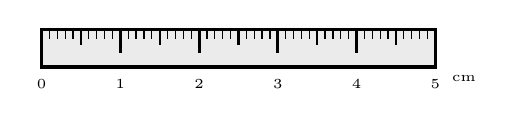
\begin{tikzpicture}[x=1cm, y=1cm, every node/.style={font=\scriptsize, text=black}]
      \draw[black, line width=1.1pt, fill=panelgray] (0,0) rectangle (5.0, 0.48);
      \foreach \m in {0,...,50}{
        \pgfmathsetmacro{\xval}{\m*0.1}
        \draw[black, line width=0.45pt] (\xval, 0.48) -- (\xval, 0.36);
      }
      \foreach \h in {0,0.5,...,5.0}{
        \draw[black, line width=0.8pt] (\h, 0.48) -- (\h, 0.28);
      }
      \foreach \c in {0,1,2,3,4,5}{
        \draw[black, line width=1.1pt] (\c, 0.48) -- (\c, 0.18);
        \node[below=1pt, font=\tiny] at (\c, 0.0) {\en{\c}};
      }
      \node[right=2pt, font=\tiny] at (5.02, -0.14) {\en{cm}};
    \end{tikzpicture}
  \end{tcolorbox}
\end{minipage}

\vspace{4pt}

% --- ផ្នែកទី ១៖ សកម្មភាព 1 — ត្រីកោណកែង 3-4-5 cm ពីរ + 35° SSA vs 90° (x=1cm, y=1cm) ---
\textbf{១. សកម្មភាព \en{1} ៖ កាត់ត្រីកោណ $3\text{--}4\text{--}5\unit{cm}$ ផ្គុំត្រឡប់ខ្នង ($\ang{BAB'}=180^\circ$) \& ប្រៀបធៀបធ្នូ \en{SSA} $35^\circ$ \en{vs} កែង $90^\circ$ (\en{x=1cm, y=1cm})}

\vspace{2pt}
\noindent
{\centering
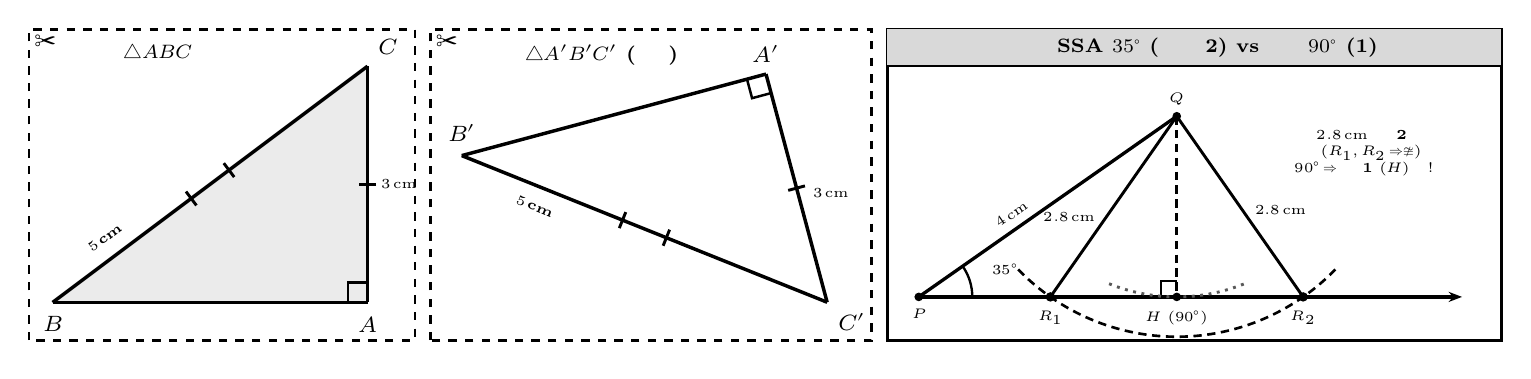
\begin{tikzpicture}[x=1cm, y=1cm, every node/.style={font=\scriptsize, text=black}]
  % === ឆ្វេង៖ កាត់ ១ — ∆ABC (AB=4cm, AC=3cm, BC=5cm, ∠A=90°) ===
  \begin{scope}[shift={(0,0)}]
    \draw[black, dashed, line width=0.95pt] (0, 0) rectangle (4.90, 3.95);
    \node[anchor=north west, inner sep=1pt, font=\footnotesize] at (0.03, 3.92) {\scissors};
    \node[anchor=north west, font=\scriptsize] at (0.45, 3.88) {\textbf{កាត់ ១៖ $\tri{ABC}$}};
    \coordinate (A) at (4.30, 0.48);
    \coordinate (B) at (0.30, 0.48);
    \coordinate (C) at (4.30, 3.48);
    \fill[panelgray] (A) -- (B) -- (C) -- cycle;
    \draw[black, line width=1.25pt] (A) -- (B);
    \draw[black, line width=1.25pt, tk1] (A) -- (C);
    \draw[black, line width=1.25pt, tk2] (B) -- (C);
    \pic[draw=black, line width=0.9pt, angle radius=2.5mm]{right angle=B--A--C};
    \node[below=1.5pt, font=\footnotesize] at (A) {$A$};
    \node[below=1.5pt, font=\footnotesize] at (B) {$B$};
    \node[above right=0.5pt, font=\footnotesize] at (C) {$C$};
    \node[right=1.5pt, font=\tiny] at ($(A)!0.50!(C)$) {$3\unit{cm}$};
    \node[above left=1.5pt, rotate=36.87, font=\tiny] at ($(B)!0.28!(C)$) {\textbf{$5\unit{cm}$}};
  \end{scope}

  % === កណ្ដាល៖ កាត់ ២ — ∆A'B'C' ឆ្លុះ និងបង្វិល 195° ===
  \begin{scope}[shift={(5.10, 0)}]
    \draw[black, dashed, line width=0.95pt] (0, 0) rectangle (5.60, 3.95);
    \node[anchor=north west, inner sep=1pt, font=\footnotesize] at (0.03, 3.92) {\scissors};
    \node[anchor=north west, font=\scriptsize] at (0.45, 3.88) {\textbf{កាត់ ២៖ $\tri{A'B'C'}$ (បង្វិល)}};
    \coordinate (Ap) at (4.26, 3.38);
    \coordinate (Bp) at (0.3963, 2.3447);
    \coordinate (Cp) at (5.0365, 0.4822);
    \fill[white] (Ap) -- (Bp) -- (Cp) -- cycle;
    \draw[black, line width=1.25pt] (Ap) -- (Bp);
    \draw[black, line width=1.25pt, tk1] (Ap) -- (Cp);
    \draw[black, line width=1.25pt, tk2] (Bp) -- (Cp);
    \pic[draw=black, line width=0.9pt, angle radius=2.5mm]{right angle=Cp--Ap--Bp};
    \node[above=0.5pt, font=\footnotesize] at (Ap) {$A'$};
    \node[above=1.5pt, font=\footnotesize] at (Bp) {$B'$};
    \node[below right=0.5pt, font=\footnotesize] at (Cp) {$C'$};
    \node[right=2pt, font=\tiny] at ($(Ap)!0.52!(Cp)$) {$3\unit{cm}$};
    \node[below left=1.5pt, rotate=-21.87, font=\tiny] at ($(Bp)!0.30!(Cp)$) {\textbf{$5\unit{cm}$}};
  \end{scope}

  % === ស្ដាំ៖ ប្រៀបធៀប 35° SSA (PQ=4cm, r=2.8cm -> 2 ចំណុច R1, R2) vs ប៉ះកែង 90° (H) ===
  \begin{scope}[shift={(10.90, 0)}]
    \draw[black, line width=1.1pt] (0, 0) rectangle (7.80, 3.95);
    \fill[headgray] (0, 3.48) rectangle (7.80, 3.95);
    \draw[black, line width=0.9pt] (0, 3.48) -- (7.80, 3.48);
    \node[font=\scriptsize] at (3.90, 3.71) {\textbf{អន្ទាក់ \en{SSA} $35^\circ$ (ប្រសព្វ \en{2}) \en{vs} ប៉ះកែង $90^\circ$ (\en{1})}};
    % 1:1 exact coords: P=(0.40,0.55), Q=(3.6766,2.8443), R1=(2.0716,0.55), R2=(5.2817,0.55), H=(3.6766,0.55)
    \coordinate (P) at (0.40, 0.55);
    \coordinate (X) at (7.30, 0.55);
    \coordinate (Q) at (3.6766, 2.8443);
    \coordinate (R1) at (2.0716, 0.55);
    \coordinate (R2) at (5.2817, 0.55);
    \coordinate (H) at (3.6766, 0.55);
    \draw[black, line width=1.2pt, -{Stealth[length=1.7mm]}] (P) -- (X);
    \draw[black, line width=1.2pt] (P) -- (Q);
    \draw[black, line width=1.05pt] (Q) -- (R1);
    \draw[black, line width=1.05pt] (Q) -- (R2);
    \draw[black, densely dashed, line width=1.0pt] (Q) -- (H);
    \pic[draw=black, line width=0.8pt, angle radius=2.0mm]{right angle=P--H--Q};
    % Arc r=2.8 cm centered at Q from -136 deg to -44 deg
    \draw[black, densely dashed, line width=0.95pt] ($(Q)+(-136:2.8)$) arc (-136:-44:2.8);
    % Tangent arc r=2.2943 cm centered at Q from -112 deg to -68 deg
    \draw[darkline, dotted, line width=1.05pt] ($(Q)+(-112:2.2943)$) arc (-112:-68:2.2943);
    \pic[draw=black, line width=0.85pt, angle radius=6.8mm]{angle=X--P--Q};
    \node[font=\tiny] at ($(P)+(17.5:1.15)$) {$35^\circ$};
    \node[above left=0pt, rotate=35, font=\tiny] at ($(P)!0.48!(Q)$) {$4\unit{cm}$};
    \node[left=0.5pt, font=\tiny] at ($(Q)!0.56!(R1)$) {$2.8\unit{cm}$};
    \node[right=1pt, font=\tiny] at ($(Q)!0.52!(R2)$) {$2.8\unit{cm}$};
    \fill[black] (P) circle (0.055) node[below=1pt, font=\tiny] {$P$};
    \fill[black] (Q) circle (0.055) node[above=0.5pt, font=\tiny] {$Q$};
    \fill[black] (R1) circle (0.06) node[below=1.5pt, font=\tiny] {$R_1$};
    \fill[black] (H) circle (0.055) node[below=1.5pt, font=\tiny] {$H$ ($90^\circ$)};
    \fill[black] (R2) circle (0.06) node[below=1.5pt, font=\tiny] {$R_2$};
    \node[anchor=west, font=\tiny, align=left] at (5.05, 2.38) {ធ្នូ $2.8\unit{cm}$ កាត់ \textbf{2}\\ចំណុច ($R_1,R_2 \Rightarrow \ncg$)\\$90^\circ \Rightarrow$ ប៉ះ \textbf{1} ($H$) គត់!};
  \end{scope}
\end{tikzpicture}\par}

\vspace{3pt}

% --- ផ្ទាំងផ្គុំត្រឡប់ខ្នង 1:1 (x=1cm, y=1cm) + កំណត់ត្រា POE 1 ---
\noindent
\begin{minipage}[c]{9.4cm}
  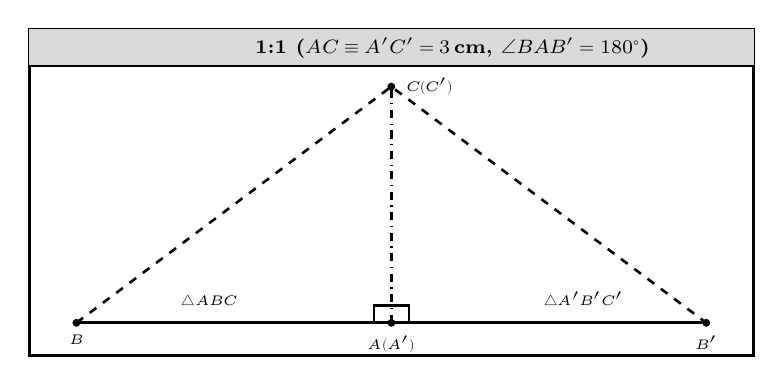
\begin{tikzpicture}[x=1cm, y=1cm, every node/.style={font=\scriptsize, text=black}]
    \draw[black, line width=1.05pt, fill=white] (0,0) rectangle (9.20, 4.15);
    \fill[headgray] (0, 3.68) rectangle (9.20, 4.15);
    \draw[black, line width=0.85pt] (0, 3.68) -- (9.20, 3.68);
    \node[font=\scriptsize] at (4.60, 3.91) {\textbf{ផ្ទាំងផ្គុំត្រឡប់ខ្នង \en{1:1} ($AC \equiv A'C'=3\unit{cm}$, $\ang{BAB'}=180^\circ$)}};
    \coordinate (MA) at (4.60, 0.42);
    \coordinate (MB) at (0.60, 0.42);
    \coordinate (MBp) at (8.60, 0.42);
    \coordinate (MC) at (4.60, 3.42);
    \draw[black, line width=1.2pt] (MB) -- (MBp);
    \draw[black, dashed, line width=0.95pt] (MB) -- (MC) -- (MBp);
    \draw[black, dash dot, line width=1.05pt] (MA) -- (MC);
    \pic[draw=black, line width=0.8pt, angle radius=2.2mm]{right angle=MB--MA--MC};
    \pic[draw=black, line width=0.8pt, angle radius=2.2mm]{right angle=MC--MA--MBp};
    \fill[black] (MA) circle (0.05) node[below=1pt, font=\tiny] {$A(A')$};
    \fill[black] (MB) circle (0.05) node[below=1pt, font=\tiny] {$B$};
    \fill[black] (MBp) circle (0.05) node[below=1pt, font=\tiny] {$B'$};
    \fill[black] (MC) circle (0.05) node[right=2pt, font=\tiny] {$C(C')$};
    \node[above right=1pt, font=\tiny] at (1.50, 0.48) {ដាក់ $\tri{ABC}$};
    \node[above left=1pt, font=\tiny] at (7.70, 0.48) {ដាក់ $\tri{A'B'C'}$};
  \end{tikzpicture}
\end{minipage}%
\hfill
\begin{minipage}[c]{9.45cm}
  \begin{tcolorbox}[
    enhanced, sharp corners, colback=panelgray, colframe=black,
    boxrule=1.0pt, boxsep=1pt, top=4pt, bottom=4pt, left=5pt, right=5pt,
    title={\textbf{កំណត់ត្រា \en{POE 1} ៖ ត្រឡប់ខ្នង \en{HL} \en{vs} អន្ទាក់ \en{SSA} $35^\circ$}},
    colbacktitle=headgray, coltitle=black, fonttitle=\fontsize{8.2pt}{11pt}\selectfont
  ]
    \raggedright\fontsize{7.95pt}{11.5pt}\selectfont
    \textbf{\en{P} \en{--} ទស្សន៍ទាយ៖} បើផ្គុំជ្រុង $A'C'$ ត្រួតជាប់ខ្នង $AC$ តើបន្ទាត់ $B\text{--}A\text{--}B'$ ជាបន្ទាត់ត្រង់តែមួយទេ? \chkbox\ ត្រង់ \chkbox\ កាច់កែង\\[3pt]
    \textbf{POE ១ (សង្កេតត្រឡប់ខ្នង $3\text{--}4\text{--}5$ \en{vs} $35^\circ$ \en{SSA})៖}\\
    $\bullet$ $\ang{BAB'} = 90^\circ + 90^\circ = \underline{\hspace{0.8cm}}^\circ \Rightarrow B, A, B'$ រួមបន្ទាត់ត្រង់!\\
    $\bullet$ $CB = CB' = 5\unit{cm} \Rightarrow \tri{BCB'}$ សមបាទ $\Rightarrow \ang{B} = \ang{\underline{\hspace{0.45cm}}}$!\\[3pt]
    \textbf{\en{E} \en{--} ពន្យល់៖} ហេតុអ្វី $90^\circ$ ប៉ះ/ចាក់សោត្រីកោណតែ \textbf{១ គត់} ខុសពី $35^\circ$ (កាត់ $R_1, R_2$)?\\[2pt]
    \rule{\linewidth}{0.55pt}
  \end{tcolorbox}
\end{minipage}

\vspace{4pt}

% --- ផ្នែកទី ២៖ សកម្មភាព 2 (POE 2) — គំរូបត់ពុះមុំត្រីកោណសាមញ្ញ (Scalene) 1:1 ---
\textbf{២. សកម្មភាព \en{2} (\en{POE 2}) ៖ កាត់បត់ពុះមុំត្រីកោណសាមញ្ញ ($\tri{ABC}$) រកប្រសព្វ $I$ \& វាស់រង្វង់ក្នុង (\en{x=1cm, y=1cm})}

\vspace{2pt}
\noindent
\begin{minipage}[c]{10.45cm}
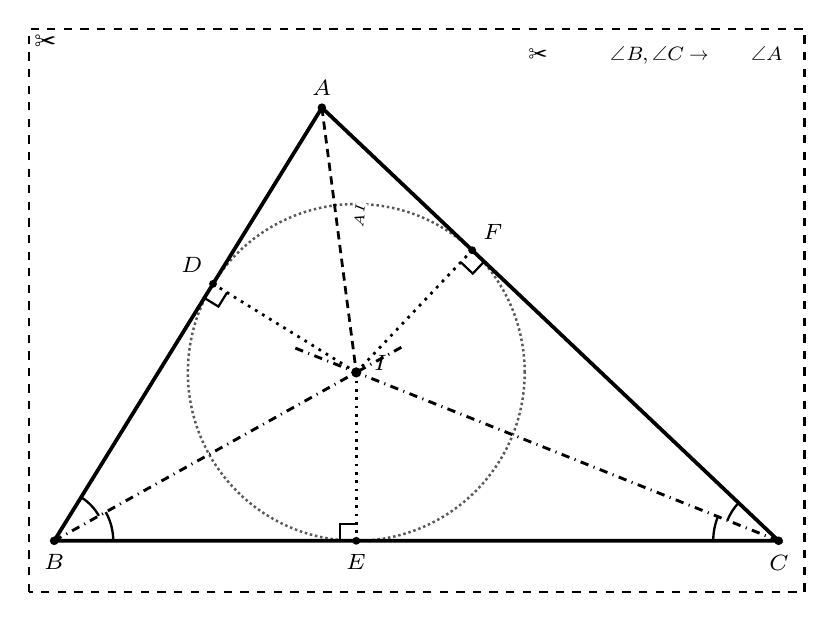
\begin{tikzpicture}[x=1cm, y=1cm, every node/.style={font=\scriptsize, text=black}]
  % Cut box: 9.85 cm x 7.15 cm (fits cleanly inside 10.45 cm minipage with zero overfull!)
  \draw[black, dashed, line width=0.95pt] (0, 0) rectangle (9.85, 7.15);
  \node[anchor=north west, inner sep=1pt, font=\footnotesize] at (0.03, 7.12) {\scissors};
  \node[anchor=north east, font=\scriptsize] at (9.70, 7.05) {កាត់ \scissors{} រួចបត់ពុះ $\ang{B}, \ang{C} \rightarrow$ តេស្ត $\ang{A}$};

  % Exact 1:1 scalene ∆ABC: B=(0.32, 0.65), C=(9.52, 0.65), A=(3.72, 6.15) (BC=9.2 cm exact!)
  % I=(4.1565, 2.7887), r=2.1387, D=(2.3373, 3.9133), E=(4.1565, 0.65), F=(5.6281, 4.3406)
  \coordinate (B) at (0.32, 0.65);
  \coordinate (C) at (9.52, 0.65);
  \coordinate (A) at (3.72, 6.15);
  \coordinate (I) at (4.1565, 2.7887);
  \coordinate (D) at (2.3373, 3.9133);
  \coordinate (E) at (4.1565, 0.65);
  \coordinate (F) at (5.6281, 4.3406);

  % Faint inscribed circle test guide
  \draw[darkline, densely dotted, line width=0.9pt] (I) circle (2.1387);

  % Solid scalene triangle
  \draw[black, line width=1.35pt] (A) -- (B) -- (C) -- cycle;

  % Angle B and C bisector fold lines meeting at I
  \draw[black, dash dot, line width=1.05pt] (B) -- ($(B)!1.15!(I)$);
  \draw[black, dash dot, line width=1.05pt] (C) -- ($(C)!1.15!(I)$);
  % Dashed test fold line AI (no angle arcs at A!)
  \draw[black, densely dashed, line width=1.0pt] (A) -- (I);

  % Perpendicular drops ID, IE, IF
  \draw[black, dotted, line width=1.0pt] (I) -- (D);
  \draw[black, dotted, line width=1.0pt] (I) -- (E);
  \draw[black, dotted, line width=1.0pt] (I) -- (F);
  \pic[draw=black, line width=0.8pt, angle radius=2.1mm]{right angle=B--D--I};
  \pic[draw=black, line width=0.8pt, angle radius=2.1mm]{right angle=B--E--I};
  \pic[draw=black, line width=0.8pt, angle radius=2.1mm]{right angle=C--F--I};

  % Bisector arcs ONLY at B (single) and C (double) -- CCW interior order!
  \pic[draw=black, line width=0.85pt, angle radius=6.5mm]{angle=I--B--A};
  \pic[draw=black, line width=0.85pt, angle radius=7.5mm]{angle=C--B--I};
  \pic[draw=black, line width=0.85pt, angle radius=7.0mm]{angle=A--C--I};
  \pic[draw=black, line width=0.85pt, angle radius=8.3mm]{angle=I--C--B};

  \fill[black] (A) circle (0.055) node[above=1pt, font=\footnotesize] {$A$};
  \fill[black] (B) circle (0.055) node[below=1.5pt, font=\footnotesize] {$B$};
  \fill[black] (C) circle (0.055) node[below=1.5pt, font=\footnotesize] {$C$};
  \fill[black] (I) circle (0.065);
  \node[font=\footnotesize, inner sep=0.5pt] at ($(I)+(0.30, 0.12)$) {$I$};
  \fill[black] (D) circle (0.05) node[above left=0.5pt, font=\footnotesize] {$D$};
  \fill[black] (E) circle (0.05) node[below=1.5pt, font=\footnotesize] {$E$};
  \fill[black] (F) circle (0.05) node[above right=0.5pt, font=\footnotesize] {$F$};
  \node[font=\tiny, rotate=83, fill=white, inner sep=0.6pt] at ($(A)!0.48!(I)+(0.24,0)$) {តេស្តបត់ $AI$};
\end{tikzpicture}
\end{minipage}%
\hfill
\begin{minipage}[c]{8.35cm}
  \begin{tcolorbox}[
    enhanced, sharp corners, colback=white, colframe=black,
    boxrule=1.05pt, boxsep=1pt, top=4pt, bottom=4pt, left=5pt, right=5pt,
    title={\textbf{កំណត់ត្រា \en{POE 2} ៖ ផ្ចិតរង្វង់ក្នុង $I$ ($ID=IE=IF$ \en{vs} $IA,IB,IC$)}},
    colbacktitle=headgray, coltitle=black, fonttitle=\fontsize{8.0pt}{11pt}\selectfont
  ]
    \raggedright\fontsize{7.85pt}{11.4pt}\selectfont
    \textbf{\en{P} \en{--} ទស្សន៍ទាយ៖} បត់ពុះ $\ang{B}$ និង $\ang{C}$ ប្រសព្វត្រង់ $I$ តើបន្ទាត់បត់ពុះ $\ang{A}$ នឹងកាត់ត្រង់ $I$ ដែរទេ?\\
    \chkbox\ កាត់ត្រង់ $I$ \hspace{0.4cm} \chkbox\ មិនកាត់\\[4pt]
    \textbf{\en{O} \en{--} សង្កេត (បត់ផ្ទៀង \& វាស់បន្ទាត់ខ្នាត \en{1:1 cm})៖}\\[2pt]
    \renewcommand{\arraystretch}{1.15}
    \begin{tabular}{|L{2.20cm}|L{3.20cm}|L{1.32cm}|}
      \hline
      \cellcolor{panelgray}\textbf{ប្រភេទចម្ងាយ} & \cellcolor{panelgray}\textbf{រង្វាស់បន្ទាត់ (\en{cm})} & \cellcolor{panelgray}\textbf{សង្កេត} \\ \hline
      \textbf{កែងទៅជ្រុង ៣}\newline (កាំរង្វង់ក្នុង) & $ID=\underline{\hspace{0.58cm}}$, $IE=\underline{\hspace{0.58cm}}$,\newline $IF=\underline{\hspace{0.58cm}}$ & \chkbox\ ស្មើ\newline \chkbox\ ខុស \\ \hline
      \textbf{ទៅកំពូល ៣}\newline (អន្ទាក់!) & $IA=\underline{\hspace{0.58cm}}$, $IB=\underline{\hspace{0.58cm}}$,\newline $IC=\underline{\hspace{0.58cm}}$ & \chkbox\ ស្មើ\newline \chkbox\ ខុស \\ \hline
    \end{tabular}\\[4pt]
    \textbf{\en{E} \en{--} ពន្យល់ (សរុប \en{E2})៖} ហេតុអ្វីផ្ចិត $I$ ប៉ះជ្រុងទាំង ៣ ($ID=IE=IF$) តែ $IA, IB, IC$ មិនស្មើគ្នា?\\[2pt]
    \rule{\linewidth}{0.55pt}\\[11pt]
    \rule{\linewidth}{0.55pt}
  \end{tcolorbox}
\end{minipage}

\clearpage

% ============================================================================
% ទំព័រទី ២៖ E4 Elaborate — កាត "ផែនទីច្រវាក់ អ.ម -> អ.ជ ផ្ចិត I" (២ ប័ណ្ណ)
% CRITICAL: SCALENE ∆ABC, DASHED AI, ZERO '/' on AD, BD, BE, AF, ZERO arcs at ∠A!
% ============================================================================
\pagebanner{សម្ភារៈទី ២៖ កាត \enbf{E4} «ផែនទីច្រវាក់ អ\enbf{.}ម \enbf{\ensuremath{\rightarrow}} អ\enbf{.}ជ ផ្ចិត \enbf{I}»}{ទំព័រ ២/៦ \en{-- E4 Elaborate} (កាត់ ២ ប័ណ្ណ \scissors)}

\newcommand{\eFourCardHL}[1]{%
\begin{tcolorbox}[
  enhanced, sharp corners, colback=white, colframe=white,
  borderline={1.0pt}{0pt}{black, dashed},
  boxsep=1pt, top=3.5pt, bottom=3.5pt, left=5pt, right=5pt
]
  \begin{tcolorbox}[
    enhanced, sharp corners, colback=headgray, colframe=black,
    boxrule=0.8pt, boxsep=1pt, top=2.5pt, bottom=2.5pt, left=5pt, right=5pt, after skip=4.5pt
  ]
    \fontsize{8.3pt}{11.2pt}\selectfont
    \textbf{\scissors\ កាតសកម្មភាព \en{E4} (#1) \en{--} ផែនទីច្រវាក់ អ.ម \en{$\rightarrow$} អ.ជ ផ្ចិត $I$} \hfill ក្រុម៖ $\underline{\hspace{2.8cm}}$
  \end{tcolorbox}

  \noindent
  \begin{minipage}[t]{7.55cm}
    \vspace{0pt}
    \fontsize{7.95pt}{11.2pt}\selectfont
    \textbf{លំហាត់គំរូ (ទំព័រ ១៥៥)៖} កន្លះបន្ទាត់ពុះនៃ $\ang{B}$ និង $\ang{C}$ ក្នុងត្រីកោណ $ABC$ ប្រសព្វគ្នាត្រង់ $I$~។ តាម $I$ គូសបន្ទាត់កែងនឹង $AB, BC, AC$ ត្រង់ $D, E, F$ រៀងគ្នា~។ \textbf{ក.} បង្ហាញថា $ID=IE=IF$~។ \textbf{ខ.} បង្ហាញថា $AI$ ជាកន្លះបន្ទាត់ពុះនៃ $\ang{BAC}$~។
    \begin{center}
    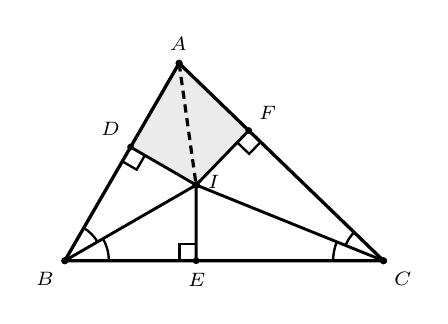
\begin{tikzpicture}[scale=0.88, every node/.style={font=\scriptsize, text=black}]
      % CLEAN SCALENE ∆ABC (BC=4.6, AC=4.102, AB=3.293)
      % ZERO '/' ticks on AD, BD, BE, AF! ZERO arcs at ∠A! DASHED AI!
      \coordinate (B) at (0, 0);
      \coordinate (C) at (4.60, 0);
      \coordinate (A) at (1.65, 2.85);
      \coordinate (I) at (1.8957, 1.0930);
      \coordinate (D) at (0.9498, 1.6406);
      \coordinate (E) at (1.8957, 0);
      \coordinate (F) at (2.6551, 1.8790);

      \fill[panelgray] (A) -- (D) -- (I) -- (F) -- cycle;
      \draw[black, line width=1.2pt] (A) -- (B) -- (C) -- cycle;
      \draw[black, line width=1.05pt] (B) -- (I) (C) -- (I);
      % DASHED AI (construction line, no angle arcs at A!)
      \draw[black, densely dashed, line width=1.15pt] (A) -- (I);
      % Perpendicular drops ID, IE, IF
      \draw[black, line width=1.05pt] (I) -- (D) (I) -- (E) (I) -- (F);

      % Right angles ONLY at D, E, F
      \pic[draw=black, line width=0.85pt, angle radius=2.1mm]{right angle=B--D--I};
      \pic[draw=black, line width=0.85pt, angle radius=2.1mm]{right angle=B--E--I};
      \pic[draw=black, line width=0.85pt, angle radius=2.1mm]{right angle=C--F--I};

      % Bisector arcs ONLY at B (single) and C (double) -- CCW interior order!
      \pic[draw=black, line width=0.85pt, angle radius=4.8mm]{angle=I--B--A};
      \pic[draw=black, line width=0.85pt, angle radius=5.6mm]{angle=C--B--I};
      \pic[draw=black, line width=0.85pt, angle radius=5.2mm]{angle=A--C--I};
      \pic[draw=black, line width=0.85pt, angle radius=6.4mm]{angle=I--C--B};

      \fill[black] (A) circle (1.5pt) node[above=1pt] {$A$};
      \fill[black] (B) circle (1.5pt) node[below left=0.5pt] {$B$};
      \fill[black] (C) circle (1.5pt) node[below right=0.5pt] {$C$};
      \fill[black] (I) circle (1.6pt);
      \node[anchor=west, inner sep=0.6pt] at ($(I)+(0.14, 0.05)$) {$I$};
      \fill[black] (D) circle (1.4pt) node[above left=0.5pt] {$D$};
      \fill[black] (E) circle (1.4pt) node[below=1pt] {$E$};
      \fill[black] (F) circle (1.4pt) node[above right=0.5pt] {$F$};
    \end{tikzpicture}
    \end{center}
    \begin{tcolorbox}[enhanced, sharp corners, colback=panelgray, colframe=black, boxrule=0.7pt, boxsep=1pt, top=2.5pt, bottom=2.5pt, left=4pt, right=4pt]
      \raggedright\fontsize{7.4pt}{10.5pt}\selectfont
      \textbf{ពិនិត្យក្រោយ (\en{EIA} ៣០ វិនាទី)៖} យើងស្រាយបាន $ID=IE=IF$ (ចម្ងាយពី $I$ ទៅជ្រុង ៣)។ តើ $IA=IB=IC$ ដែរឬទេ? \chkbox\ មិនស្មើ (ព្រោះ $\tri{ABC}$ សាមញ្ញ!)\\
      ហេតុអ្វី\textbf{ហាមគូស} \tickone\ លើ $AD, BD, BE, AF$ មុនស្រាយ? ($\underline{\hspace{1.9cm}}$)
    \end{tcolorbox}
  \end{minipage}\hfill
  \begin{minipage}[t]{10.25cm}
    \vspace{0pt}
    \begin{tcolorbox}[enhanced, sharp corners, colback=white, colframe=black, boxrule=0.85pt, boxsep=1pt, top=3pt, bottom=3pt, left=5pt, right=5pt]
      \raggedright\fontsize{7.85pt}{11.3pt}\selectfont
      \textbf{ដំណាក់កាល ១ [អូសម្រាមដៃ \en{[tracing]} $BI, CI \Rightarrow$ អ.ម $\times 2 \Rightarrow ID=IE=IF$]៖}\\
      \chkbox\ គូស $90^\circ$ ត្រង់ $D, E, F$ (\cnum{1}) + ធ្នូពុះមុំត្រង់ $B, C$ (\textbf{គ្មាន \tickone\ លើ $AD, AF$!})\\
      $\bullet$ $\tri{BEI}\cg\tri{BDI}$ (អ.ម \en{HA} ព្រោះ $BI$ រួម, $\ang{IBE}=\ang{IBD}$) $\Rightarrow ID = \underline{\hspace{0.60cm}}$ \en{(1)}\\
      $\bullet$ $\tri{CEI}\cg\tri{CFI}$ (អ.ម \en{HA} ព្រោះ $CI$ រួម, $\ang{ICE}=\ang{ICF}$) $\Rightarrow IE = \underline{\hspace{0.60cm}}$ \en{(2)}\\
      $\Rightarrow$ តាម \en{(1)} និង \en{(2)} គេបាន $\mathbf{ID = IE = IF}$ \textit{(បញ្ជូនទៅដំណាក់កាល ២!)}
    \end{tcolorbox}
    \vspace{2.5pt}
    \begin{tcolorbox}[enhanced, sharp corners, colback=panelgray, colframe=black, boxrule=0.85pt, boxsep=1pt, top=3pt, bottom=3pt, left=5pt, right=5pt]
      \raggedright\fontsize{7.85pt}{11.3pt}\selectfont
      \textbf{ដំណាក់កាល ២ [អូសម្រាមដៃ \en{[tracing]} $AI$ ឈម $90^\circ \Rightarrow$ អ.ជ (\en{HL})]៖}\\
      ក្នុងត្រីកោណកែង $IDA$ និងត្រីកោណកែង $IFA$ មាន៖\\
      \en{1)} $\ang{IDA} = \ang{\underline{\hspace{0.75cm}}} = 90^\circ$ \hspace{0.2cm} (\cnum{1} $ID\perp AB, IF\perp AC$)\\
      \en{2)} អ៊ីប៉ូតេនុសរួម $AI = \underline{\hspace{0.65cm}}$ \hspace{0.2cm} (\cnum{2} ឈម $90^\circ$)\\
      \en{3)} ជ្រុងមុំកែង $ID = \underline{\hspace{0.65cm}}$ \hspace{0.2cm} (\cnum{3} លទ្ធផល \textbf{ក.} ខាងលើ)\\
      ដូចនេះ $\tri{IDA} \cg \tri{\underline{\hspace{0.75cm}}}$ (\cnum{4} $\underline{\hspace{1.40cm}}$) $\Rightarrow \ang{IAD} = \ang{\underline{\hspace{0.75cm}}}$ (\cnum{5}) $\Rightarrow AI$ ពុះ $\ang{BAC}$!
    \end{tcolorbox}
    \vspace{2.5pt}
    \raggedright{\fontsize{7.0pt}{9.8pt}\selectfont
    \textbf{ធនាគារអំណះអំណាង (\en{HL})៖} \cnum{1} មុំកែង $90^\circ$ \en{|} \cnum{2} អ៊ីប៉ូតេនុសស្មើ/រួម \en{|} \cnum{3} ជ្រុងមុំកែងស្មើ/រួម \en{|} \cnum{4} អ.ជ (\en{HL}) \en{|} \cnum{5} ធាតុត្រូវគ្នា/ច្រាសពុះមុំ\par}
  \end{minipage}
\end{tcolorbox}%
}

\eFourCardHL{ប័ណ្ណទី ១}

\vspace{6pt}
\noindent\scissors\ \dotfill\ \textbf{កាត់តាមស្នាមចុចចែកជា ២ ប័ណ្ណ (\en{Cut Along Dashed Line})} \dotfill\ \scissors
\vspace{6pt}

\eFourCardHL{ប័ណ្ណទី ២}

\clearpage

% ============================================================================
% ទំព័រទី ៣៖ E5 Evaluate — "តុសវនកម្មចំណុចកណ្ដាល-អង្កត់កែង ៣ តួនាទី" (២ សន្លឹក)
% ============================================================================
\pagebanner{សម្ភារៈទី ៣៖ «តុសវនកម្មចំណុចកណ្ដាល\enbf{--}អង្កត់កែង ៣ តួនាទី» \enbf{(E5 \& E1)}}{ទំព័រ ៣/៦ \en{-- E5 Evaluate} (កាត់ ២ សន្លឹក \scissors)}

\newcommand{\eFiveSheetHL}[1]{%
\begin{tcolorbox}[
  enhanced, sharp corners, colback=white, colframe=white,
  borderline={1.0pt}{0pt}{black, dashed},
  boxsep=1pt, top=3pt, bottom=3pt, left=4.5pt, right=4.5pt
]
  \begin{tcolorbox}[
    enhanced, sharp corners, colback=headgray, colframe=black,
    boxrule=0.8pt, boxsep=1pt, top=2pt, bottom=2pt, left=5pt, right=5pt, after skip=3.5pt
  ]
    \fontsize{7.7pt}{10.5pt}\selectfont
    \textbf{\scissors\ តុសវនកម្មចំណុចកណ្ដាល\en{--}អង្កត់កែង (#1) \en{--} ក្រុម៖} $\underline{\hspace{1.7cm}}$ \hfill \textbf{ប្រតិបត្តិ (ទំ.១៥៦)៖} $M$ កណ្ដាល $BC$, $MD\perp AB, ME\perp AC, MD=ME \Rightarrow \ang{B}=\ang{C}$
  \end{tcolorbox}

  \renewcommand{\arraystretch}{1.04}
  {\centering\setlength{\tabcolsep}{3.5pt}%
  \begin{tabular}{|L{6.30cm}|L{5.75cm}|L{5.55cm}|}
    \hline
    \cellcolor{panelgray}\centering\arraybackslash\fontsize{7.5pt}{10.0pt}\selectfont\textbf{តួនាទី ១៖ គូសសញ្ញា \en{\&} បំបែកត្រីកោណ}\newline {\fontsize{6.9pt}{9.1pt}\selectfont \textbf{\en{Pause-Ask!}} \en{--} ព្រួញ $90^\circ \to$ អ៊ីប៉ូតេនុស $MB=MC$} &
    \cellcolor{panelgray}\centering\arraybackslash\fontsize{7.5pt}{10.0pt}\selectfont\textbf{តួនាទី ២៖ សម្រាយ ៣ បន្ទាត់ \& \cnum{1}--\cnum{4}}\newline {\fontsize{6.9pt}{9.1pt}\selectfont សរសេរលក្ខខណ្ឌ \textbf{អ.ជ (\en{HL})} ភ្ជាប់លេខ} &
    \cellcolor{panelgray}\centering\arraybackslash\fontsize{7.5pt}{10.0pt}\selectfont\textbf{តួនាទី ៣៖ វិបាក \cnum{5} \& បិទ \en{E1}}\newline {\fontsize{6.9pt}{9.1pt}\selectfont \textbf{\en{Pause-Review!}} $\ang{B}=\ang{C}$ \en{+} ស្រះរង្វង់} \\ \hline

    % --- Column 1: Book p.156 Pratibat figure + Exploded ∆MDB, ∆MEC silhouettes ---
    {\centering
    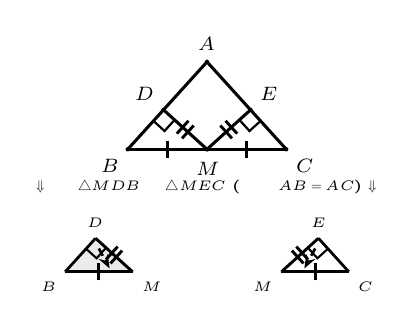
\begin{tikzpicture}[scale=0.61, every node/.style={font=\scriptsize, text=black}]
      % Main ∆ABC: B=(-1.65,0), C=(1.65,0), A=(0,1.82), M=(0,0), D=(-0.9056,0.8210), E=(0.9056,0.8210)
      \coordinate (B) at (-1.65, 0);
      \coordinate (C) at (1.65, 0);
      \coordinate (A) at (0, 1.82);
      \coordinate (M) at (0, 0);
      \coordinate (D) at (-0.9056, 0.8210);
      \coordinate (E) at (0.9056, 0.8210);
      \draw[black, line width=1.1pt] (B) -- (A) -- (C);
      \draw[black, line width=1.15pt, tk1] (B) -- (M);
      \draw[black, line width=1.15pt, tk1] (M) -- (C);
      \draw[black, line width=1.1pt, tk2] (M) -- (D);
      \draw[black, line width=1.1pt, tk2] (M) -- (E);
      \pic[draw=black, line width=0.8pt, angle radius=1.9mm]{right angle=B--D--M};
      \pic[draw=black, line width=0.8pt, angle radius=1.9mm]{right angle=C--E--M};
      \fill[black] (A) circle (1.3pt) node[above=0.5pt] {$A$};
      \fill[black] (B) circle (1.3pt) node[below left=0pt] {$B$};
      \fill[black] (C) circle (1.3pt) node[below right=0pt] {$C$};
      \fill[black] (M) circle (1.4pt) node[below=1pt] {$M$};
      \fill[black] (D) circle (1.3pt) node[above left=0pt] {$D$};
      \fill[black] (E) circle (1.3pt) node[above right=0pt] {$E$};

      \node[font=\tiny] at (0, -0.78) {$\Downarrow$ \textbf{បំបែក $\tri{MDB}$ និង $\tri{MEC}$ (ហាមសន្មត $AB=AC$)} $\Downarrow$};
      % Exploded ∆MDB (shifted left)
      \begin{scope}[shift={(-1.55, -2.55)}, scale=0.85]
        \coordinate (B1) at (-1.65, 0); \coordinate (M1) at (0, 0); \coordinate (D1) at (-0.9056, 0.8210);
        \fill[panelgray] (B1) -- (M1) -- (D1) -- cycle;
        \draw[black, line width=1.05pt, tk1] (B1) -- (M1);
        \draw[black, line width=1.05pt, tk2] (M1) -- (D1);
        \draw[black, line width=1.0pt] (B1) -- (D1);
        \pic[draw=black, line width=0.75pt, angle radius=1.8mm]{right angle=B1--D1--M1};
        \draw[hypArrow] ($(D1)+(0.08,-0.25)$) -- ($(B1)!0.66!(M1)+(0,0.08)$);
        \node[below left=0pt, font=\tiny] at (B1) {$B$};
        \node[below right=0pt, font=\tiny] at (M1) {$M$};
        \node[above=0.5pt, font=\tiny] at (D1) {$D$};
      \end{scope}
      % Exploded ∆MEC (shifted right)
      \begin{scope}[shift={(1.55, -2.55)}, scale=0.85]
        \coordinate (M2) at (0, 0); \coordinate (C2) at (1.65, 0); \coordinate (E2) at (0.9056, 0.8210);
        \fill[white] (M2) -- (C2) -- (E2) -- cycle;
        \draw[black, line width=1.05pt, tk1] (M2) -- (C2);
        \draw[black, line width=1.05pt, tk2] (M2) -- (E2);
        \draw[black, line width=1.0pt] (E2) -- (C2);
        \pic[draw=black, line width=0.75pt, angle radius=1.8mm]{right angle=C2--E2--M2};
        \draw[hypArrow] ($(E2)+(-0.08,-0.25)$) -- ($(M2)!0.34!(C2)+(0,0.08)$);
        \node[below left=0pt, font=\tiny] at (M2) {$M$};
        \node[below right=0pt, font=\tiny] at (C2) {$C$};
        \node[above=0.5pt, font=\tiny] at (E2) {$E$};
      \end{scope}
    \end{tikzpicture}\par}
    \fontsize{7.0pt}{9.6pt}\selectfont
    \chkbox\ គូស $90^\circ$ ត្រង់ $D, E$, \tickone\ លើ $BM=MC$, \ticktwo\ លើ $MD=ME$, ព្រួញ $90^\circ \to MB, MC$\\
    \chkbox\ \textbf{\en{Pause-Ask!}} «ហេតុអ្វី $MB, MC$ ជាអ៊ីប៉ូតេនុស និងហាមសន្មតតាមភ្នែកថា $AB=AC$?»
    &
    % --- Column 2: Proof ①–④ ---
    \fontsize{7.5pt}{11.1pt}\selectfont
    ក្នុងត្រីកោណកែង $\tri{MDB}$ និង $\tri{MEC}$ មាន៖\par\vspace{3pt}
    \en{1)} $\ang{MDB} = \ang{\underline{\hspace{0.75cm}}} = 90^\circ$ (\cnum{1} $\underline{\hspace{1.15cm}}$)\par\vspace{3pt}
    \en{2)} អ៊ីប៉ូតេនុស $MB = \underline{\hspace{0.65cm}}$ (\cnum{2} $M$ កណ្ដាល $BC$)\par\vspace{3pt}
    \en{3)} ជ្រុងមុំកែង $MD = \underline{\hspace{0.65cm}}$ (\cnum{3} $\underline{\hspace{1.15cm}}$)\par\vspace{4pt}
    ដូចនេះ $\tri{MDB} \cg \tri{\underline{\hspace{0.75cm}}}$ (\cnum{4} $\underline{\hspace{1.15cm}}$)\par\vspace{6pt}
    \begin{tcolorbox}[enhanced, sharp corners, colback=panelgray, colframe=black, boxrule=0.6pt, boxsep=1pt, top=3pt, bottom=3pt, left=4pt, right=4pt]
      \raggedright\fontsize{6.85pt}{9.7pt}\selectfont
      \textbf{ចំណាំប្រយ័ត្ន៖} រូបទំ.១៥៦ មើលទៅស៊ីមេទ្រីដូចសមបាទ ប៉ុន្តែ\textbf{មិនទាន់ដឹង} $AB=AC$ ទេ — ត្រូវប្រើ \textbf{អ.ជ (\en{HL})} ជាមុន!\\[2pt]
      \textbf{ធនាគារ៖} \cnum{1} មុំកែង $90^\circ$ \en{|} \cnum{2} អ៊ីប៉ូតេនុស \en{|} \cnum{3} ជ្រុងកែង \en{|} \cnum{4} អ.ជ
    \end{tcolorbox}
    &
    % --- Column 3: Pause-Review, ∠B=∠C & E1 Closure ---
    \fontsize{7.4pt}{10.9pt}\selectfont
    \chkbox\ \textbf{\en{Pause-Review!}} ផ្ទៀងលំដាប់កំពូល៖\newline
    $M\leftrightarrow M,\; D\leftrightarrow\underline{\hspace{0.35cm}}\; (90^\circ),\; B\leftrightarrow\underline{\hspace{0.35cm}}$\par\vspace{3pt}
    \textbf{វិបាក (\cnum{5})៖} $\ang{B} = \ang{\underline{\hspace{0.55cm}}}$ (មុំត្រូវគ្នានៃត្រីកោណប៉ុនគ្នា!)\par\vspace{5pt}
    \begin{tcolorbox}[enhanced, sharp corners, colback=panelgray, colframe=black, boxrule=0.7pt, boxsep=1pt, top=3pt, bottom=3pt, left=4pt, right=4pt]
      \raggedright\fontsize{6.9pt}{9.8pt}\selectfont
      \textbf{បិទបេសកកម្ម \en{E1} (អាងទឹករង្វង់សួនផ្លូវ ៣ ខ្សែ)៖}\\
      $\bullet$ ប្រសព្វពុះ $\ang{B}, \ang{C}$ ត្រង់ $I \xrightarrow{\text{អ.ម}} ID=IE=IF$ (ស្មើចម្ងាយផ្លូវ ៣ ខ្សែ!)\\
      $\bullet$ ផ្ទៀង $ID=IF$ \& $AI$ រួម $\xrightarrow{\text{អ.ជ}}$ (\cnum{4}) $AI$ ពុះ $\ang{A}$ (\cnum{5}) $\Rightarrow$ ផ្ចិតស្រះ $I$ តែមួយ!
    \end{tcolorbox}
    \\[1pt] \hline
  \end{tabular}\par}
\end{tcolorbox}%
}

\eFiveSheetHL{សន្លឹកទី ១}

\vspace{5pt}
\noindent\scissors\ \dotfill\ \textbf{កាត់តាមស្នាមចុចចែកជា ២ សន្លឹក (\en{Cut Along Dashed Line})} \dotfill\ \scissors
\vspace{5pt}

\eFiveSheetHL{សន្លឹកទី ២}

\clearpage

% ============================================================================
% ទំព័រទី ៤៖ ផ្ទាំងយោងប្រចាំថ្នាក់រៀន — ទ្រឹស្ដីបទ អ.ជ (HL), ប្រសព្វពុះមុំ & ធនាគារ ①–⑤
% ============================================================================
\begin{tcolorbox}[
  enhanced, sharp corners, colback=white, colframe=black,
  boxrule=1.5pt, borderline={0.6pt}{2.2pt}{black},
  boxsep=1pt, top=4pt, bottom=4pt, left=6pt, right=6pt
]
  \begin{center}
    {\muol\fontsize{11.4pt}{16pt}\selectfont ទ្រឹស្ដីបទ អ\enbf{.}ជ \enbf{(HL) ,} ប្រសព្វពុះមុំក្នុង និងធនាគារ \cnum{1}\enbf{--}\cnum{5}}\\[1pt]
    {\fontsize{8.5pt}{11.8pt}\selectfont ផ្ទាំងយោងប្រចាំថ្នាក់រៀន (ស-ខ្មៅ) \en{--} មេរៀនទី១២ (១.៣.២) អ៊ីប៉ូតេនុសប៉ុនគ្នា និងជ្រុងមុំកែងមួយប៉ុនគ្នា}\\[2pt]
    \khmflourish
  \end{center}
  \vspace{1pt}

  % --- ផ្នែកទី ១៖ ទ្រឹស្ដីបទ អ.ជ (HL) + រូបត្រឡប់ខ្នងស៊ីចង្វាក់ AC=A'C', BC=B'C' ---
  \noindent
  \begin{minipage}[c]{8.55cm}
    \begin{tcolorbox}[enhanced, sharp corners, colback=panelgray, colframe=black, boxrule=0.85pt, boxsep=1pt, top=3.5pt, bottom=3.5pt, left=5pt, right=5pt]
      \raggedright\fontsize{7.9pt}{11.3pt}\selectfont
      \textbf{ទ្រឹស្ដីបទ (អ.ជ / \en{HL} \en{--} ទំ.១៥៥)៖} ត្រីកោណកែងពីរប៉ុនគ្នាកាលណាវាមាន \textbf{អ៊ីប៉ូតេនុសប៉ុនគ្នា} និង \textbf{ជ្រុងនៃមុំកែងមួយប៉ុនគ្នា}~។\\[2.5pt]
      \textbf{វិធីចងចាំ៖} គូសប្រអប់ $90^\circ \rightarrow$ ព្រួញទៅអ៊ីប៉ូតេនុស ($BC=B'C'$) $+$ ជ្រុងកែង ១ ($AC=A'C'$) $\Rightarrow$ \textbf{ត្រឡប់ខ្នងផ្គុំ} ឃើញ $\ang{BAB'}=180^\circ$!
    \end{tcolorbox}
  \end{minipage}\hfill
  \begin{minipage}[c]{9.25cm}
    \centering
    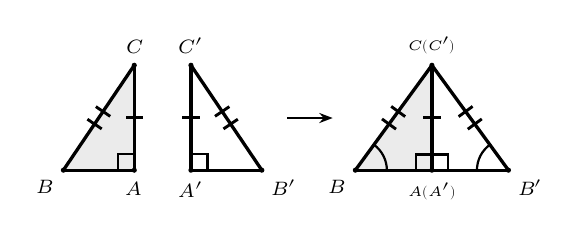
\begin{tikzpicture}[scale=0.72, every node/.style={font=\scriptsize, text=black}]
      % Left: Separate ∆ABC and ∆A'B'C' (Consistent AC=A'C' with '|', BC=B'C' with '||')
      \coordinate (A) at (1.25, 0.0); \coordinate (B) at (0.0, 0.0); \coordinate (C) at (1.25, 1.85);
      \fill[panelgray] (A) -- (B) -- (C) -- cycle;
      \draw[black, line width=1.1pt] (A) -- (B);
      \draw[black, line width=1.2pt, tk1] (A) -- (C);
      \draw[black, line width=1.2pt, tk2] (B) -- (C);
      \pic[draw=black, line width=0.8pt, angle radius=2.1mm]{right angle=B--A--C};
      \fill[black] (A) circle (1.3pt) (B) circle (1.3pt) (C) circle (1.3pt);
      \node[below=0.5pt] at (A) {$A$}; \node[below left=0pt] at (B) {$B$}; \node[above=0.5pt] at (C) {$C$};

      \coordinate (Ap) at (2.25, 0.0); \coordinate (Bp) at (3.50, 0.0); \coordinate (Cp) at (2.25, 1.85);
      \fill[white] (Ap) -- (Bp) -- (Cp) -- cycle;
      \draw[black, line width=1.1pt] (Ap) -- (Bp);
      \draw[black, line width=1.2pt, tk1] (Ap) -- (Cp);
      \draw[black, line width=1.2pt, tk2] (Bp) -- (Cp);
      \pic[draw=black, line width=0.8pt, angle radius=2.1mm]{right angle=Cp--Ap--Bp};
      \fill[black] (Ap) circle (1.3pt) (Bp) circle (1.3pt) (Cp) circle (1.3pt);
      \node[below=0.5pt] at (Ap) {$A'$}; \node[below right=0pt] at (Bp) {$B'$}; \node[above=0.5pt] at (Cp) {$C'$};

      \draw[black, line width=1.0pt, -{Stealth[length=1.7mm]}] (3.95, 0.92) -- (4.75, 0.92);
      \node[above=1pt, font=\tiny] at (4.35, 0.95) {ផ្គុំខ្នង};

      % Right: Joined isosceles ∆BCB'
      \coordinate (JA) at (6.50, 0.0); \coordinate (JB) at (5.15, 0.0); \coordinate (JBp) at (7.85, 0.0); \coordinate (JC) at (6.50, 1.85);
      \fill[panelgray] (JA) -- (JB) -- (JC) -- cycle;
      \draw[black, line width=1.15pt] (JB) -- (JBp);
      \draw[black, line width=1.2pt, tk1] (JA) -- (JC);
      \draw[black, line width=1.2pt, tk2] (JB) -- (JC);
      \draw[black, line width=1.2pt, tk2] (JBp) -- (JC);
      \pic[draw=black, line width=0.8pt, angle radius=2.0mm]{right angle=JB--JA--JC};
      \pic[draw=black, line width=0.8pt, angle radius=2.0mm]{right angle=JC--JA--JBp};
      \pic[draw=black, line width=0.8pt, angle radius=4.0mm]{angle=JA--JB--JC};
      \pic[draw=black, line width=0.8pt, angle radius=4.0mm]{angle=JC--JBp--JA};
      \fill[black] (JA) circle (1.3pt) (JB) circle (1.3pt) (JBp) circle (1.3pt) (JC) circle (1.3pt);
      \node[below=1pt, font=\tiny] at (JA) {$A(A')$}; \node[below left=0pt] at (JB) {$B$}; \node[below right=0pt] at (JBp) {$B'$}; \node[above=0.5pt, font=\tiny] at (JC) {$C(C')$};
    \end{tikzpicture}
  \end{minipage}

  \vspace{3.5pt}

  % --- ផ្នែកទី ២៖ កែកំហុសទាំង ៣ ទំព័រ ១៥៤ + ទ្រឹស្ដីបទប្រសព្វពុះមុំក្នុង I (ទំព័រ ១៥៦) ---
  \noindent
  \begin{minipage}[t]{9.25cm}
    \begin{tcolorbox}[enhanced, sharp corners, colback=white, colframe=black, boxrule=0.95pt, boxsep=1pt, equal height group=posterMidHL, top=3pt, bottom=3pt, left=5pt, right=5pt]
      \raggedright\fontsize{7.45pt}{10.7pt}\selectfont
      \textbf{\ding{46}\ សម្រាយ \en{HL $\to$ HA} \& កែកំហុសទាំង ៣ ចំណុចទំព័រ ១៥៤៖}\\
      ក្នុង $\tri{ABC}, \tri{A'B'C'}$ មាន $\ang{A}=\ang{A'}=90^\circ$, $\mathbf{AC=A'C'}$ \textit{(កែ ១a!)}, $BC=B'C'$~។\\
      ត្រឡប់ដាក់ $A'C'$ ត្រួតលើ $AC \Rightarrow \ang{BAB'}=90^\circ+90^\circ=180^\circ$ ($BB'$ ត្រង់)~។\\
      $\tri{BCB'}$ មាន $CB=CB' \Rightarrow$ សមបាទកំពូល $C \Rightarrow \ang{B}=\ang{B'}$~។\\
      ក្នុង $\tri{BAC}, \tri{B'AC}$ មាន $\begin{cases}CB = CB' \text{ (សម្មតិកម្ម)}\\ \ang{B} = \ang{B'} \text{ (ខាងលើ)}\end{cases} \Rightarrow \tri{ABC}\cg\tri{A'B'C'}$ \textbf{(តាមលក្ខខណ្ឌ អ.ម)}!\\
      {\fontsize{7.0pt}{9.6pt}\selectfont\textit{កែ ១b--១c៖} ដូរពីរង្វង់តក្ក «\en{(}តាមលកខណ្ឌ អ\en{.}ជ\en{)}» ទៅ \textbf{«\en{(}តាមលក្ខខណ្ឌ អ\en{.}ម\en{)}»}!}
    \end{tcolorbox}
  \end{minipage}\hfill
  \begin{minipage}[t]{8.55cm}
    \begin{tcolorbox}[enhanced, sharp corners, colback=panelgray, colframe=black, boxrule=0.95pt, boxsep=1pt, equal height group=posterMidHL, top=3pt, bottom=3pt, left=5pt, right=5pt]
      \raggedright\fontsize{7.45pt}{10.7pt}\selectfont
      \textbf{ទ្រឹស្ដីបទប្រសព្វពុះមុំក្នុង (ទំព័រ ១៥៦)៖}\\[2pt]
      \begin{minipage}[c]{4.55cm}
        \raggedright\fontsize{7.25pt}{10.3pt}\selectfont
        កន្លះបន្ទាត់ពុះមុំក្នុងទាំងបីនៃត្រីកោណមួយប្រសព្វគ្នាត្រង់ចំណុចតែមួយ $I$ ដែលឋិតនៅ\textbf{ស្មើចម្ងាយពីជ្រុងទាំងបី}៖\\
        $\mathbf{ID = IE = IF}$ (ផ្ចិតរង្វង់ក្នុង)!
      \end{minipage}\hfill
      \begin{minipage}[c]{3.25cm}
        \centering
        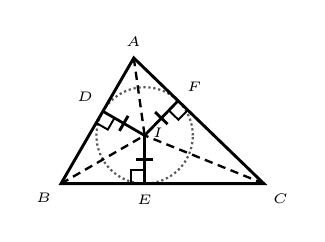
\begin{tikzpicture}[scale=0.56, every node/.style={font=\tiny, text=black}]
          \coordinate (B) at (0,0); \coordinate (C) at (4.60,0); \coordinate (A) at (1.65, 2.85);
          \coordinate (I) at (1.8957, 1.0930);
          \coordinate (D) at (0.9498, 1.6406); \coordinate (E) at (1.8957,0); \coordinate (F) at (2.6551, 1.8790);
          \draw[darkline, densely dotted, line width=0.8pt] (I) circle (1.0930);
          \draw[black, line width=1.05pt] (A)--(B)--(C)--cycle;
          \draw[black, densely dashed, line width=0.85pt] (A)--(I) (B)--(I) (C)--(I);
          \draw[black, line width=1.0pt, tk1] (I)--(D);
          \draw[black, line width=1.0pt, tk1] (I)--(E);
          \draw[black, line width=1.0pt, tk1] (I)--(F);
          \pic[draw=black, line width=0.7pt, angle radius=1.7mm]{right angle=B--D--I};
          \pic[draw=black, line width=0.7pt, angle radius=1.7mm]{right angle=B--E--I};
          \pic[draw=black, line width=0.7pt, angle radius=1.7mm]{right angle=C--F--I};
          \node[above=0.5pt] at (A) {$A$}; \node[below left=0pt] at (B) {$B$}; \node[below right=0pt] at (C) {$C$};
          \node[anchor=west, inner sep=0.4pt] at ($(I)+(0.16, 0.06)$) {$I$};
          \node[above left=0pt] at (D) {$D$}; \node[below=0.5pt] at (E) {$E$}; \node[above right=0pt] at (F) {$F$};
        \end{tikzpicture}
      \end{minipage}
    \end{tcolorbox}
  \end{minipage}

  \vspace{3.5pt}

  % --- ផ្នែកទី ៣៖ តារាងធនាគារអំណះអំណាង ①–⑤ (អ.ជ / HL & ប្រសព្វពុះមុំ) ---
  \fontsize{7.75pt}{10.7pt}\selectfont
  \renewcommand{\arraystretch}{1.05}
  \begin{tabular}{|C{0.70cm}|L{4.10cm}|L{6.45cm}|C{4.95cm}|}
    \hline
    \cellcolor{headgray}\textbf{លេខ} &
    \cellcolor{headgray}\centering\arraybackslash\textbf{ឈ្មោះអំណះអំណាង} &
    \cellcolor{headgray}\centering\arraybackslash\textbf{និមិត្តសញ្ញា និងរបៀបប្រើ} &
    \cellcolor{headgray}\centering\arraybackslash\textbf{រូបសម្គាល់ ស-ខ្មៅ} \\ \hline

    \cnum{1} &
    \textbf{មុំកែង $90^\circ$}\newline (បម្រាប់ / កម្ពស់ / កែង) &
    $\ang{A}=\ang{A'}=90^\circ$, $ID\perp AB, IF\perp AC$, $MD\perp AB$, $BD\perp AC$~។ &
    \raisebox{-0.35\height}{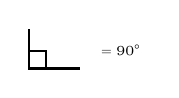
\begin{tikzpicture}[scale=0.50, every node/.style={font=\tiny, text=black}]
      \coordinate (o) at (0,0); \coordinate (a) at (1.3,0); \coordinate (b) at (0,1.0);
      \draw[black, line width=1.0pt] (b) -- (o) -- (a);
      \pic[draw=black, line width=0.8pt, angle radius=2.2mm]{right angle=a--o--b};
      \node[right=2pt] at (1.45,0.45) {$=90^\circ$};
    \end{tikzpicture}} \\ \hline

    \cnum{2} &
    \textbf{អ៊ីប៉ូតេនុសស្មើ ឬរួម}\newline (ឈម $90^\circ$) &
    $BC=B'C'$, $BM=MC$, អ៊ីប៉ូតេនុសរួម $AI=AI$, $BC=BC$, $AB=AB$~។ &
    \raisebox{-0.35\height}{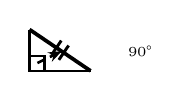
\begin{tikzpicture}[scale=0.50, every node/.style={font=\tiny, text=black}]
      \coordinate (a) at (0,0); \coordinate (b) at (1.55,0); \coordinate (c) at (0,1.05);
      \draw[black, line width=0.9pt] (c)--(a)--(b);
      \draw[black, line width=1.35pt, tk2] (b)--(c);
      \pic[draw=black, line width=0.8pt, angle radius=1.9mm]{right angle=b--a--c};
      \draw[hypArrow] (0.20,0.20) -- (0.82,0.50);
      \node[right=2pt] at (1.75,0.50) {ឈម $90^\circ$};
    \end{tikzpicture}} \\ \hline

    \cnum{3} &
    \textbf{ជ្រុងមុំកែងស្មើ ឬរួម}\newline (ជាប់ $90^\circ$) &
    $AC=A'C'$, $ID=IF$ (ពី \textbf{អ.ម}), $MD=ME$, $BD=CE$~។ &
    \raisebox{-0.35\height}{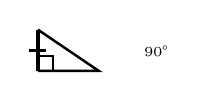
\begin{tikzpicture}[scale=0.50, every node/.style={font=\tiny, text=black}]
      \coordinate (a) at (0,0); \coordinate (b) at (1.55,0); \coordinate (c) at (0,1.05);
      \draw[black, line width=0.9pt] (a)--(b)--(c);
      \draw[black, line width=1.4pt, tk1] (a)--(c);
      \pic[draw=black, line width=0.8pt, angle radius=1.9mm]{right angle=b--a--c};
      \node[right=2pt] at (1.75,0.50) {ជាប់ $90^\circ$};
    \end{tikzpicture}} \\ \hline

    \cnum{4} &
    \textbf{លក្ខខណ្ឌ អ.ជ (\en{HL})}\newline (ឬ អ.ម ក្នុងជំហាន ១) &
    អ៊ីប៉ូតេនុស $+$ ជ្រុងមុំកែង ១ ប៉ុនគ្នា $\Rightarrow \tri{ABC}\cg\tri{A'B'C'}$~។ &
    \raisebox{-0.35\height}{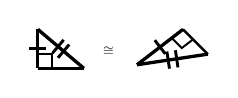
\begin{tikzpicture}[scale=0.45, every node/.style={font=\tiny, text=black}]
      \coordinate (a) at (0,0); \coordinate (b) at (1.3,0); \coordinate (c) at (0,1.1);
      \draw[black, line width=0.9pt] (a)--(b); \draw[black, line width=1.2pt, tk1] (a)--(c); \draw[black, line width=1.2pt, tk2] (b)--(c);
      \pic[draw=black, line width=0.7pt, angle radius=1.8mm]{right angle=b--a--c};
      \node at (2.0,0.5) {$\cg$};
      \coordinate (d) at (4.1,1.1); \coordinate (e) at (4.8,0.4); \coordinate (f) at (2.8,0.1);
      \draw[black, line width=0.9pt] (d)--(e); \draw[black, line width=1.2pt, tk1] (d)--(f); \draw[black, line width=1.2pt, tk2] (e)--(f);
      \pic[draw=black, line width=0.7pt, angle radius=1.8mm]{right angle=f--d--e};
    \end{tikzpicture}} \\ \hline

    \cnum{5} &
    \textbf{ធាតុត្រូវគ្នា / ច្រាសពុះមុំ} &
    $ID=IF \Rightarrow \ang{IAD}=\ang{IAF}$ ($AI$ ពុះ $\ang{A}$); $\ang{B}=\ang{C}$; $BC=AD$~។ &
    \raisebox{-0.35\height}{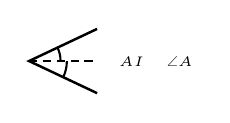
\begin{tikzpicture}[scale=0.48, every node/.style={font=\tiny, text=black}]
      \coordinate (a) at (0,0); \coordinate (b) at (1.8,0.85); \coordinate (c) at (1.8,-0.85); \coordinate (i) at (1.7,0);
      \draw[black, line width=0.9pt] (b)--(a)--(c); \draw[black, densely dashed, line width=1.0pt] (a)--(i);
      \pic[draw=black, line width=0.75pt, angle radius=4.0mm]{angle=i--a--b};
      \pic[draw=black, line width=0.75pt, angle radius=4.8mm]{angle=c--a--i};
      \node[right=2pt] at (2.0,0) {$AI$ ពុះ $\ang{A}$};
    \end{tikzpicture}} \\ \hline
  \end{tabular}

  \vspace{3.5pt}

  % --- ផ្នែកទី ៤៖ ប្រអប់ព្រមាន "អន្ទាក់ ជ.ជ.ម (60°) vs អ.ជ (90°)" & "ID=IE=IF != IA,IB,IC" ---
  \noindent
  \begin{minipage}[t]{8.75cm}
    \begin{tcolorbox}[
      enhanced, sharp corners, colback=white, colframe=black,
      boxrule=1.15pt, boxsep=1pt, equal height group=posterwarnHL,
      top=3pt, bottom=3pt, left=5pt, right=5pt,
      title={\ding{55}\ \textbf{អន្ទាក់ទី ១៖ ជ.ជ.ម ($60^\circ$) \en{vs} អ.ជ ($90^\circ$)}},
      colbacktitle=midgray, coltitle=black, fonttitle=\fontsize{8.1pt}{11pt}\selectfont
    ]
      \centering
      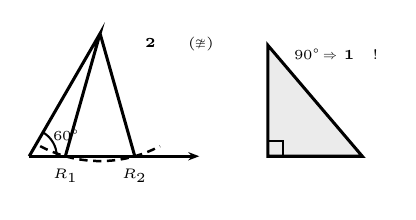
\begin{tikzpicture}[scale=0.60, every node/.style={font=\scriptsize, text=black}]
        % Left: 60 deg trap (PQ=3, Q=(1.5, 2.598), r=2.70 cuts base at R1=(0.765,0), R2=(2.235,0))
        \coordinate (P) at (0,0); \coordinate (X) at (3.6,0); \coordinate (Q) at (1.5, 2.598);
        \coordinate (R1) at (0.765,0); \coordinate (R2) at (2.235,0);
        \draw[black, line width=1.0pt, -{Stealth[length=1.4mm]}] (P)--(X);
        \draw[black, line width=1.1pt] (P)--(Q)--(R1) (Q)--(R2);
        \draw[black, densely dashed, line width=0.9pt] ($(Q)+(-118:2.70)$) arc (-118:-62:2.70);
        \pic[draw=black, line width=0.75pt, angle radius=3.5mm]{angle=X--P--Q};
        \node[font=\tiny] at (0.78, 0.44) {$60^\circ$};
        \node[below=1pt, font=\tiny] at (R1) {$R_1$}; \node[below=1pt, font=\tiny] at (R2) {$R_2$};
        \node[font=\tiny] at (2.95, 2.38) {កាត់ \textbf{2} ចំណុច ($\ncg$)};
        % Right: 90 deg unique
        \coordinate (A) at (5.05,0); \coordinate (B) at (7.05,0); \coordinate (C) at (5.05, 2.35);
        \fill[panelgray] (A)--(B)--(C)--cycle;
        \draw[black, line width=1.1pt] (A)--(B)--(C)--cycle;
        \pic[draw=black, line width=0.75pt, angle radius=1.9mm]{right angle=B--A--C};
        \node[font=\tiny] at (6.50, 2.15) {$90^\circ \Rightarrow$ \textbf{1} គត់!};
      \end{tikzpicture}
      \par\vspace{1.5pt}\fontsize{7.55pt}{10.6pt}\selectfont
      មុំស្រួច ($60^\circ$) បង្កើតត្រីកោណ \textbf{2} ខុសគ្នា (\textbf{អន្ទាក់ \en{SSA}})~។ មានតែ \textbf{$90^\circ$ (អ.ជ / \en{HL})} ទើបធានាប៉ុនគ្នា ១០០\%!
    \end{tcolorbox}
  \end{minipage}\hfill
  \begin{minipage}[t]{8.75cm}
    \begin{tcolorbox}[
      enhanced, sharp corners, colback=white, colframe=black,
      boxrule=1.15pt, boxsep=1pt, equal height group=posterwarnHL,
      top=3pt, bottom=3pt, left=5pt, right=5pt,
      title={\ding{55}\ \textbf{អន្ទាក់ទី ២៖ $ID=IE=IF \neq IA, IB, IC$}},
      colbacktitle=midgray, coltitle=black, fonttitle=\fontsize{8.1pt}{11pt}\selectfont
    ]
      \centering
      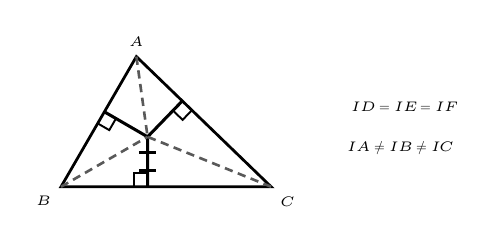
\begin{tikzpicture}[scale=0.58, every node/.style={font=\scriptsize, text=black}]
        \coordinate (B) at (0,0); \coordinate (C) at (4.60,0); \coordinate (A) at (1.65, 2.85);
        \coordinate (I) at (1.8957, 1.0930);
        \coordinate (D) at (0.9498, 1.6406); \coordinate (E) at (1.8957,0); \coordinate (F) at (2.6551, 1.8790);
        \draw[black, line width=1.0pt] (A)--(B)--(C)--cycle;
        \draw[black, line width=1.1pt, tk2] (I)--(D) (I)--(E) (I)--(F);
        \draw[darkline, densely dashed, line width=0.95pt] (A)--(I) (B)--(I) (C)--(I);
        \pic[draw=black, line width=0.7pt, angle radius=1.7mm]{right angle=B--D--I};
        \pic[draw=black, line width=0.7pt, angle radius=1.7mm]{right angle=B--E--I};
        \pic[draw=black, line width=0.7pt, angle radius=1.7mm]{right angle=C--F--I};
        \node[above=0pt, font=\tiny] at (A) {$A$}; \node[below left=0pt, font=\tiny] at (B) {$B$}; \node[below right=0pt, font=\tiny] at (C) {$C$};
        \node[right=1pt, font=\tiny] at (5.1, 1.75) {ស្មើជ្រុង៖ $ID=IE=IF$};
        \node[right=1pt, font=\tiny] at (5.1, 0.85) {ខុសកំពូល៖ $IA \neq IB \neq IC$};
      \end{tikzpicture}
      \par\vspace{1.5pt}\fontsize{7.55pt}{10.6pt}\selectfont
      ផ្ចិត $I$ ស្មើចម្ងាយពី \textbf{ជ្រុង ៣} ($ID=IE=IF$) តែ\textbf{មិនស្មើ}ពីកំពូល $A, B, C$ ទេ! (\textbf{ហាមគូស} \tickone\ លើ $AD, AF$!)
    \end{tcolorbox}
  \end{minipage}
\end{tcolorbox}

\clearpage

% ============================================================================
% ទំព័រទី ៥៖ កាតវិនិច្ឆ័យរហ័ស ៦០–៩០ វិនាទី "កាត A–D" & ចម្លើយគ្រូ — E5 Evaluate
% ============================================================================
\pagebanner{សម្ភារៈទី ៥៖ កាតវិនិច្ឆ័យរហ័ស «កាត \enbf{A--D}» \enbf{(60--90} វិនាទី\enbf{) \&} ចម្លើយគ្រូ}{ទំព័រ ៥/៦ \en{-- E5 Evaluate}}

{\fontsize{8.5pt}{12pt}\selectfont
\textbf{វិធីលេងក្នុងថ្នាក់៖} គ្រូលើកកាតម្ដងមួយ $\rightarrow$ សិស្សចង្អុលប្រអប់ $90^\circ$ ទៅអ៊ីប៉ូតេនុស $\rightarrow$ លើក \textbf{មេដៃឡើង (ពិត \ding{51})} ឬ \textbf{ខ្វែងដៃ (ខុស/អន្ទាក់ \ding{55})} + ម្រាម \en{1--3}។}

\vspace{4pt}

% --- ជួរទី ១៖ កាត A & កាត B ---
\noindent
\begin{tcolorbox}[
  enhanced, sharp corners, colback=white, colframe=white,
  borderline={1.0pt}{0pt}{black, dashed},
  width=9.25cm, equal height group=hlfoilrow1, nobeforeafter,
  boxsep=1pt, top=5pt, bottom=5pt, left=6pt, right=6pt
]
  \noindent\colorbox{black}{\textcolor{white}{\Large\textbf{\en{ A }}}}\hspace{0.25cm}{\fontsize{9.2pt}{12.5pt}\selectfont\textbf{កាត \en{A} ៖ អ.ជ (\en{HL}) បង្វិល $\approx 140^\circ$}}\par\vspace{2pt}
  \begin{center}
  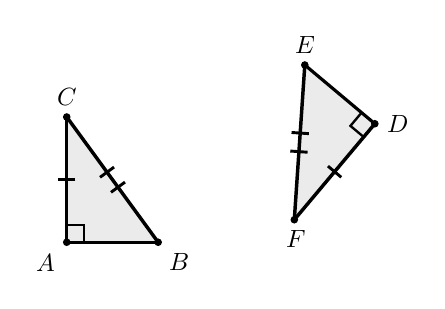
\begin{tikzpicture}[scale=0.86, every node/.style={font=\small, text=black}]
    % Upright ∆ABC
    \coordinate (A) at (0,0); \coordinate (B) at (1.35,0); \coordinate (C) at (0, 1.85);
    \fill[panelgray] (A)--(B)--(C)--cycle;
    \draw[black, line width=1.15pt] (A)--(B);
    \draw[black, line width=1.25pt, tk1] (A)--(C);
    \draw[black, line width=1.25pt, tk2] (B)--(C);
    \pic[draw=black, line width=0.85pt, angle radius=2.2mm]{right angle=B--A--C};
    \fill[black] (A) circle (1.6pt) (B) circle (1.6pt) (C) circle (1.6pt);
    \node[below left=0.5pt] at (A) {$A$}; \node[below right=0.5pt] at (B) {$B$}; \node[above=0.5pt] at (C) {$C$};
    % បង្វិល 140° ∆DEF
    \coordinate (D) at (4.55, 1.75); \coordinate (E) at (3.5158, 2.6178); \coordinate (F) at (3.3608, 0.3328);
    \fill[panelgray] (D)--(E)--(F)--cycle;
    \draw[black, line width=1.15pt] (D)--(E);
    \draw[black, line width=1.25pt, tk1] (D)--(F);
    \draw[black, line width=1.25pt, tk2] (E)--(F);
    \pic[draw=black, line width=0.85pt, angle radius=2.2mm]{right angle=F--D--E};
    \fill[black] (D) circle (1.6pt) (E) circle (1.6pt) (F) circle (1.6pt);
    \node[right=1pt] at (D) {$D$}; \node[above=0.5pt] at (E) {$E$}; \node[below=0.5pt] at (F) {$F$};
  \end{tikzpicture}
  \end{center}
  {\centering\fontsize{8.0pt}{11pt}\selectfont $\ang{A}=\ang{D}=90^\circ$, $BC=EF$ (អ៊ីប៉ូតេនុស), $AC=DF$ (ជ្រុងកែង)~។\par}
  \vfill
  \begin{tcolorbox}[enhanced, sharp corners, colback=panelgray, colframe=black, boxrule=0.8pt, boxsep=1pt, top=4pt, bottom=4pt, left=5pt, right=5pt]
    \centering\fontsize{9.0pt}{12.5pt}\selectfont
    \textbf{សំណួរ៖} តើ $\tri{ABC} \cg \tri{DEF}$ តាម \textbf{អ.ជ (\en{HL})} ឬទេ?\\[2pt]
    \chkbox\ មេដៃឡើង (\ding{51} ពិត) \hspace{0.4cm} \chkbox\ ខ្វែងដៃ (\ding{55} ខុស)
  \end{tcolorbox}
\end{tcolorbox}%
\hfill
\begin{tcolorbox}[
  enhanced, sharp corners, colback=white, colframe=white,
  borderline={1.0pt}{0pt}{black, dashed},
  width=9.25cm, equal height group=hlfoilrow1, nobeforeafter,
  boxsep=1pt, top=5pt, bottom=5pt, left=6pt, right=6pt
]
  \noindent\colorbox{black}{\textcolor{white}{\Large\textbf{\en{ B }}}}\hspace{0.25cm}{\fontsize{9.2pt}{12.5pt}\selectfont\textbf{កាត \en{B} ៖ អន្ទាក់មុំស្រួច $60^\circ$ ($60^\circ, 5\unit{cm}, 4\unit{cm}$)}}\par\vspace{2pt}
  \begin{center}
  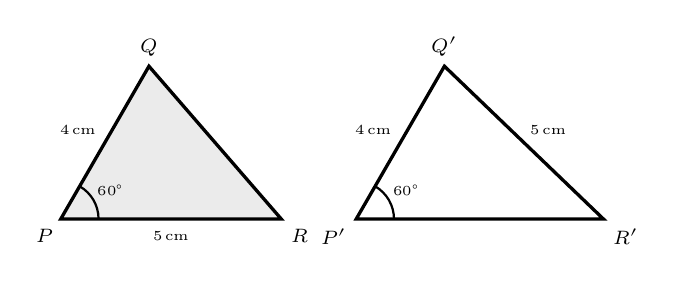
\begin{tikzpicture}[scale=0.56, every node/.style={font=\small, text=black}]
    % ∆PQR (SAS: ∠P=60°, PQ=4cm, PR=5cm)
    \coordinate (P) at (0,0); \coordinate (R) at (5.0,0); \coordinate (Q) at (2.0, 3.4641);
    \fill[panelgray] (P)--(Q)--(R)--cycle;
    \draw[black, line width=1.2pt] (P)--(Q)--(R)--cycle;
    \pic[draw=black, line width=0.8pt, angle radius=4.8mm]{angle=R--P--Q};
    \node[font=\tiny] at ($(P)+(30:1.30)$) {$60^\circ$};
    \node[above left=-1pt, font=\tiny] at (0.95, 1.75) {$4\unit{cm}$};
    \node[below=1pt, font=\tiny] at (2.5, 0) {$5\unit{cm}$};
    \node[below left=0pt, font=\scriptsize] at (P) {$P$}; \node[above=0pt, font=\scriptsize] at (Q) {$Q$}; \node[below right=0pt, font=\scriptsize] at (R) {$R$};
    % ∆P'Q'R' (SSA trap: ∠P'=60°, P'Q'=4cm, Q'R'=5cm -> P'R'=5.61cm)
    \coordinate (Pp) at (6.7,0); \coordinate (Rp) at (12.3056,0); \coordinate (Qp) at (8.7, 3.4641);
    \fill[white] (Pp)--(Qp)--(Rp)--cycle;
    \draw[black, line width=1.2pt] (Pp)--(Qp)--(Rp)--cycle;
    \pic[draw=black, line width=0.8pt, angle radius=4.8mm]{angle=Rp--Pp--Qp};
    \node[font=\tiny] at ($(Pp)+(30:1.30)$) {$60^\circ$};
    \node[above left=-1pt, font=\tiny] at (7.65, 1.75) {$4\unit{cm}$};
    \node[above right=-1pt, font=\tiny] at (10.50, 1.75) {$5\unit{cm}$};
    \node[below left=0pt, font=\scriptsize] at (Pp) {$P'$}; \node[above=0pt, font=\scriptsize] at (Qp) {$Q'$}; \node[below right=0pt, font=\scriptsize] at (Rp) {$R'$};
  \end{tikzpicture}
  \end{center}
  {\centering\fontsize{8.0pt}{11pt}\selectfont មាន $60^\circ, 4\unit{cm}, 5\unit{cm}$ ដូចគ្នា (តែគ្មាន $90^\circ$ — ជាប់ vs ឈមមុំ $60^\circ$)~។\par}
  \vfill
  \begin{tcolorbox}[enhanced, sharp corners, colback=panelgray, colframe=black, boxrule=0.8pt, boxsep=1pt, top=4pt, bottom=4pt, left=5pt, right=5pt]
    \centering\fontsize{9.0pt}{12.5pt}\selectfont
    \textbf{សំណួរ៖} តើ $\tri{PQR} \cg \tri{P'Q'R'}$ តាម \textbf{អ.ជ} ឬ \textbf{ជ.ជ.ម} ទេ?\\[2pt]
    \chkbox\ មេដៃឡើង (\ding{51} ពិត) \hspace{0.4cm} \chkbox\ ខ្វែងដៃ (\ding{55} ខុស)
  \end{tcolorbox}
\end{tcolorbox}

\vspace{6pt}

% --- ជួរទី ២៖ កាត C & កាត D ---
\noindent
\begin{tcolorbox}[
  enhanced, sharp corners, colback=white, colframe=white,
  borderline={1.0pt}{0pt}{black, dashed},
  width=9.25cm, equal height group=hlfoilrow2, nobeforeafter,
  boxsep=1pt, top=5pt, bottom=5pt, left=6pt, right=6pt
]
  \noindent\colorbox{black}{\textcolor{white}{\Large\textbf{\en{ C }}}}\hspace{0.25cm}{\fontsize{9.2pt}{12.5pt}\selectfont\textbf{កាត \en{C} ៖ អន្ទាក់ផ្ចិត $I$ ស្មើកំពូល ($IA=IB=IC$)}}\par\vspace{2pt}
  \begin{center}
  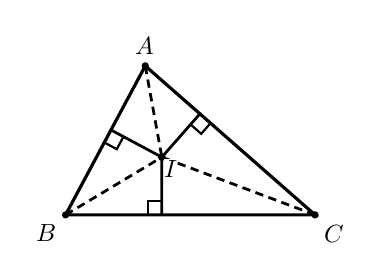
\begin{tikzpicture}[scale=0.88, every node/.style={font=\small, text=black}]
    \coordinate (B) at (0,0); \coordinate (C) at (3.60,0); \coordinate (A) at (1.15, 2.15);
    \coordinate (I) at (1.3893, 0.8325);
    \coordinate (D) at (0.6553, 1.2251); \coordinate (E) at (1.3893, 0.0); \coordinate (F) at (1.9384, 1.4581);
    \draw[black, line width=1.15pt] (A)--(B)--(C)--cycle;
    \draw[black, densely dashed, line width=1.0pt] (A)--(I) (B)--(I) (C)--(I);
    \draw[black, line width=1.0pt] (I)--(D) (I)--(E) (I)--(F);
    \pic[draw=black, line width=0.8pt, angle radius=1.8mm]{right angle=B--D--I};
    \pic[draw=black, line width=0.8pt, angle radius=1.8mm]{right angle=B--E--I};
    \pic[draw=black, line width=0.8pt, angle radius=1.8mm]{right angle=C--F--I};
    \fill[black] (A) circle (1.5pt) node[above=0.5pt] {$A$};
    \fill[black] (B) circle (1.5pt) node[below left=0pt] {$B$};
    \fill[black] (C) circle (1.5pt) node[below right=0pt] {$C$};
    \fill[black] (I) circle (1.6pt) node[below right=0.5pt, fill=white, inner sep=0.4pt] {$I$};
  \end{tikzpicture}
  \end{center}
  {\centering\fontsize{8.0pt}{11pt}\selectfont $I$ ជាប្រសព្វកន្លះបន្ទាត់ពុះមុំក្នុងនៃត្រីកោណសាមញ្ញ $ABC$~។\par}
  \vfill
  \begin{tcolorbox}[enhanced, sharp corners, colback=panelgray, colframe=black, boxrule=0.8pt, boxsep=1pt, top=4pt, bottom=4pt, left=5pt, right=5pt]
    \centering\fontsize{9.0pt}{12.5pt}\selectfont
    \textbf{សំណួរ៖} គេថា $IA = IB = IC$ (ស្មើចម្ងាយពីកំពូល ៣) ត្រូវឬខុស?\\[2pt]
    \chkbox\ មេដៃឡើង (\ding{51} ពិត) \hspace{0.4cm} \chkbox\ ខ្វែងដៃ (\ding{55} ខុស)
  \end{tcolorbox}
\end{tcolorbox}%
\hfill
\begin{tcolorbox}[
  enhanced, sharp corners, colback=white, colframe=white,
  borderline={1.0pt}{0pt}{black, dashed},
  width=9.25cm, equal height group=hlfoilrow2, nobeforeafter,
  boxsep=1pt, top=5pt, bottom=5pt, left=6pt, right=6pt
]
  \noindent\colorbox{black}{\textcolor{white}{\Large\textbf{\en{ D }}}}\hspace{0.25cm}{\fontsize{9.2pt}{12.5pt}\selectfont\textbf{កាត \en{D} ៖ អន្ទាក់អ៊ីប៉ូតេនុស $5\unit{cm}$ \en{vs} ជ្រុងកែង $5\unit{cm}$}}\par\vspace{2pt}
  \begin{center}
  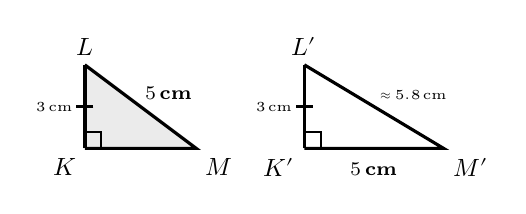
\begin{tikzpicture}[scale=0.68, every node/.style={font=\small, text=black}]
    % ∆KLM: KL=3 (1.56), KM=4 (2.08), hyp LM=5 cm
    \coordinate (K) at (0,0); \coordinate (M) at (2.08,0); \coordinate (L) at (0, 1.56);
    \fill[panelgray] (K)--(L)--(M)--cycle;
    \draw[black, line width=1.15pt] (K)--(M)--(L);
    \draw[black, line width=1.25pt, tk1] (K)--(L);
    \pic[draw=black, line width=0.8pt, angle radius=2.1mm]{right angle=M--K--L};
    \node[left=1pt, font=\tiny] at (0, 0.78) {$3\unit{cm}$};
    \node[above right=-1pt, font=\scriptsize] at (1.00, 0.78) {\textbf{$5\unit{cm}$}};
    \node[below left=0pt] at (K) {$K$}; \node[above=0pt] at (L) {$L$}; \node[below right=0pt] at (M) {$M$};
    % ∆K'L'M': K'L'=3 (1.56), leg K'M'=5 (2.60) -> hyp L'M'=5.83 cm
    \coordinate (Kp) at (4.10,0); \coordinate (Mp) at (6.70,0); \coordinate (Lp) at (4.10, 1.56);
    \fill[white] (Kp)--(Lp)--(Mp)--cycle;
    \draw[black, line width=1.15pt] (Kp)--(Mp)--(Lp);
    \draw[black, line width=1.25pt, tk1] (Kp)--(Lp);
    \pic[draw=black, line width=0.8pt, angle radius=2.1mm]{right angle=Mp--Kp--Lp};
    \node[left=1pt, font=\tiny] at (4.10, 0.78) {$3\unit{cm}$};
    \node[below=1.5pt, font=\scriptsize] at (5.40, 0) {\textbf{$5\unit{cm}$}};
    \node[above right=-1pt, font=\tiny] at (5.40, 0.78) {$\approx 5.8\unit{cm}$};
    \node[below left=0pt] at (Kp) {$K'$}; \node[above=0pt] at (Lp) {$L'$}; \node[below right=0pt] at (Mp) {$M'$};
  \end{tikzpicture}
  \end{center}
  {\centering\fontsize{8.0pt}{11pt}\selectfont $KL=K'L'=3\unit{cm}$, អ៊ីប៉ូតេនុស $LM=5\unit{cm}$ ទល់ជ្រុងកែង $K'M'=5\unit{cm}$~។\par}
  \vfill
  \begin{tcolorbox}[enhanced, sharp corners, colback=panelgray, colframe=black, boxrule=0.8pt, boxsep=1pt, top=4pt, bottom=4pt, left=5pt, right=5pt]
    \centering\fontsize{9.0pt}{12.5pt}\selectfont
    \textbf{សំណួរ៖} តើ $\tri{KLM} \cg \tri{K'L'M'}$ តាម \textbf{អ.ជ (\en{HL})} ឬទេ?\\[2pt]
    \chkbox\ មេដៃឡើង (\ding{51} ពិត) \hspace{0.4cm} \chkbox\ ខ្វែងដៃ (\ding{55} ខុស)
  \end{tcolorbox}
\end{tcolorbox}

\vspace{6pt}

% --- ខ្សែកាត់ & បន្ទះចម្លើយសម្រាប់គ្រូ ---
\noindent\scissors\ \dotfill\ \textbf{កាត់ទុកសម្រាប់គ្រូ (\en{Teacher Mini Answer \& Remediation Key})} \dotfill\ \scissors

\vspace{4pt}
\begin{tcolorbox}[
  enhanced, sharp corners, colback=panelgray, colframe=black,
  boxrule=1.0pt, boxsep=1pt, top=4pt, bottom=4pt, left=5pt, right=5pt
]
  \fontsize{7.7pt}{10.8pt}\selectfont
  \renewcommand{\arraystretch}{1.10}
  \begin{tabular}{|L{4.05cm}|L{4.25cm}|L{4.25cm}|L{4.45cm}|}
    \hline
    \cellcolor{headgray}\textbf{កាត \en{A} ៖ មេដៃឡើង (\ding{51})} &
    \cellcolor{headgray}\textbf{កាត \en{B} ៖ ខ្វែងដៃ (\ding{55})} &
    \cellcolor{headgray}\textbf{កាត \en{C} ៖ ខ្វែងដៃ (\ding{55})} &
    \cellcolor{headgray}\textbf{កាត \en{D} ៖ ខ្វែងដៃ (\ding{55})} \\ \hline
    $\tri{ABC}\cg\tri{DEF}$ តាម \textbf{អ.ជ (\en{HL})} ទោះបង្វិល $\approx 140^\circ$ ព្រោះ $90^\circ$, អ៊ីប៉ូតេនុស $BC=EF$, ជ្រុងកែង $AC=DF$! &
    \textbf{អន្ទាក់មុំស្រួច $60^\circ$ (\en{SSA})!} គ្មាន $90^\circ$ ហើយ $5\unit{cm}$ ប្ដូរទីតាំង ($PR=5$ \en{vs} $Q'R'=5 \Rightarrow P'R'\approx 5.6\unit{cm} \Rightarrow \ncg$)។ &
    \textbf{ច្រឡំផ្ចិត $I$ ទៅកំពូល!} ផ្ចិតប្រសព្វពុះមុំ $I$ ស្មើចម្ងាយពី\textbf{ជ្រុង ៣} ($ID=IE=IF$) មិនមែនពីកំពូល $IA,IB,IC$ ទេ។ &
    \textbf{អន្ទាក់អ៊ីប៉ូតេនុស \en{vs} ជ្រុងកែង!} $LM=5\unit{cm}$ ឈម $90^\circ$ តែ $K'M'=5\unit{cm}$ ជាជ្រុងកែង ($L'M'\approx 5.8\unit{cm} \Rightarrow \ncg$)។ \\ \hline
  \end{tabular}
  \par\vspace{2.5pt}
  \textbf{ត្រួតទំនុកចិត្ត (ម្រាម ១\en{--}៣)៖} ១ ម្រាម = គូសព្រួញ $90^\circ \to$ អ៊ីប៉ូតេនុសជាមួយដៃគូ \hspace{0.2cm}\en{|}\hspace{0.2cm} ២ ម្រាម = ផ្ទៀងធនាគារ \cnum{1}--\cnum{5} \hspace{0.2cm}\en{|}\hspace{0.2cm} ៣ ម្រាម = ច្បាស់ ១០០\%
\end{tcolorbox}

\clearpage

% ============================================================================
% ទំព័រទី ៦៖ ប័ណ្ណកិច្ចការផ្ទះ ជំហានទី ៥ — ៤ ប័ណ្ណក្នុង ១ ទំព័រ A4 (4-up: HW #10 & #12)
% ============================================================================
\pagebanner{សម្ភារៈទី ៦៖ ប័ណ្ណកិច្ចការផ្ទះ ជំហានទី ៥ \enbf{--} ៤ ប័ណ្ណក្នុង ១ ទំព័រ \enbf{A4}}{ទំព័រ ៦/៦ \en{--} ជំហានទី ៥ (កាត់ ៤ ប័ណ្ណ \scissors)}

% ម៉ាក្រូប័ណ្ណកិច្ចការផ្ទះ ៤-up (ផ្ទៀង ១០០% នឹងលំហាត់ទី ១០ និងទី ១២ ទំព័រ ១៦៥)
\newcommand{\hwslipFourHL}[1]{%
\begin{tcolorbox}[
  enhanced, sharp corners, colback=white, colframe=white,
  borderline={0.95pt}{0pt}{black, dashed},
  width=9.25cm, equal height group=hwquadHL, nobeforeafter,
  boxsep=1pt, top=3pt, bottom=3pt, left=4.5pt, right=4.5pt
]
  \begin{tcolorbox}[
    enhanced, sharp corners, colback=headgray, colframe=black,
    boxrule=0.7pt, boxsep=1pt, top=2pt, bottom=2pt, left=4pt, right=4pt, after skip=3.5pt
  ]
    \fontsize{7.4pt}{10.2pt}\selectfont
    \textbf{\scissors\ កិច្ចការផ្ទះ (#1) \en{|} ១.៣.២ អ.ជ (\en{HL}) \& ប្រសព្វពុះមុំ} \hfill \textbf{ចន្ទ ៣០/១១/២៦}\\[1.5pt]
    ឈ្មោះ៖ $\underline{\hspace{4.0cm}}$ \hspace{0.2cm} ថ្នាក់៖ $\underline{\hspace{1.0cm}}$
  \end{tcolorbox}

  % --- លំហាត់ទី ១០ (សៀវភៅទំព័រ ១៦៥ — បន្ថែម [AC និង AB] + បំបែក ∆BDC, ∆CEB) ---
  \noindent
  \begin{minipage}[c]{4.85cm}
    \fontsize{7.2pt}{10.2pt}\selectfont
    \textbf{លំហាត់ទី ១០ (ទំ.១៦៥)៖} $ABC$ ជាត្រីកោណមួយ~។ កម្ពស់គូសចេញពីកំពូល $B$ និង $C$ កាត់ជ្រុងឈម \textbf{[AC និង AB]} ត្រង់ $D$ និង $E$ រៀងគ្នា~។ បង្ហាញថា បើ $BD=CE$ នោះ $\ang{ABC}=\ang{ACB}$~។\\
    {\fontsize{6.6pt}{9.3pt}\selectfont\textit{តម្រុយ៖} បំបែក $\tri{BDC}$ និង $\tri{CEB}$ (អ៊ីប៉ូតេនុសរួម $BC$, $BD=CE$) $\Rightarrow$ ស្រាយតាម \textbf{អ.ជ (\en{HL})}!}
  \end{minipage}\hfill
  \begin{minipage}[c]{3.75cm}
    \centering
    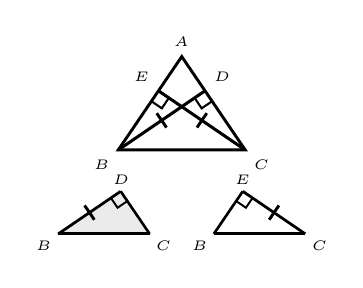
\begin{tikzpicture}[scale=0.52, every node/.style={font=\tiny, text=black}]
      % Main ∆ABC: B=(-1.55,0), C=(1.55,0), A=(0,2.28), D=(0.568,1.444), E=(-0.568,1.444)
      \coordinate (B) at (-1.55,0); \coordinate (C) at (1.55,0); \coordinate (A) at (0,2.28);
      \coordinate (D) at (0.568, 1.444); \coordinate (E) at (-0.568, 1.444);
      \draw[black, line width=1.05pt] (A)--(B)--(C)--cycle;
      \draw[black, line width=1.1pt, tk1] (B)--(D);
      \draw[black, line width=1.1pt, tk1] (C)--(E);
      \pic[draw=black, line width=0.75pt, angle radius=1.6mm]{right angle=C--D--B};
      \pic[draw=black, line width=0.75pt, angle radius=1.6mm]{right angle=B--E--C};
      \node[above=0pt] at (A) {$A$}; \node[below left=0pt] at (B) {$B$}; \node[below right=0pt] at (C) {$C$};
      \node[above right=0pt] at (D) {$D$}; \node[above left=0pt] at (E) {$E$};
      % Exploded silhouettes ∆BDC (left) and ∆CEB (right) cleanly below
      \begin{scope}[shift={(-1.90, -2.05)}, scale=0.72]
        \coordinate (b1) at (-1.55,0); \coordinate (c1) at (1.55,0); \coordinate (d1) at (0.568, 1.444);
        \fill[panelgray] (b1)--(c1)--(d1)--cycle;
        \draw[black, line width=1.0pt, tk1] (b1)--(d1);
        \draw[black, line width=1.15pt] (b1)--(c1);
        \draw[black, line width=0.95pt] (c1)--(d1);
        \pic[draw=black, line width=0.7pt, angle radius=1.5mm]{right angle=c1--d1--b1};
        \node[below left=-1pt] at (b1) {$B$}; \node[below right=-1pt] at (c1) {$C$}; \node[above=-1pt] at (d1) {$D$};
      \end{scope}
      \begin{scope}[shift={(1.90, -2.05)}, scale=0.72]
        \coordinate (b2) at (-1.55,0); \coordinate (c2) at (1.55,0); \coordinate (e2) at (-0.568, 1.444);
        \fill[white] (b2)--(c2)--(e2)--cycle;
        \draw[black, line width=1.0pt, tk1] (c2)--(e2);
        \draw[black, line width=1.15pt] (b2)--(c2);
        \draw[black, line width=0.95pt] (b2)--(e2);
        \pic[draw=black, line width=0.7pt, angle radius=1.5mm]{right angle=b2--e2--c2};
        \node[below left=-1pt] at (b2) {$B$}; \node[below right=-1pt] at (c2) {$C$}; \node[above=-1pt] at (e2) {$E$};
      \end{scope}
    \end{tikzpicture}
  \end{minipage}

  \vspace{3.5pt}
  \hrule height 0.5pt
  \vspace{3.5pt}

  % --- លំហាត់ទី ១២ (សៀវភៅទំព័រ ១៦៥ + បំបែក ∆ACB, ∆BDA) ---
  \noindent
  \begin{minipage}[c]{4.85cm}
    \fontsize{7.2pt}{10.2pt}\selectfont
    \textbf{លំហាត់ទី ១២ (ទំ.១៦៥)៖} ក្នុងរូបខាងស្ដាំ គេឱ្យ $AC=BD$ និង $\ang{C}=\ang{D}=90^\circ$~។ បង្ហាញថា $BC=AD$ និង $BC \parallel AD$~។\\
    {\fontsize{6.6pt}{9.3pt}\selectfont\textit{តម្រុយ៖} បំបែក $\tri{ACB}\cg\tri{BDA}$ (អ.ជ, $AB$ រួម) $\Rightarrow BC=AD$ និងមុំឆ្លាស់ក្នុង $\ang{CBA}=\ang{DAB}$!}
  \end{minipage}\hfill
  \begin{minipage}[c]{3.75cm}
    \centering
    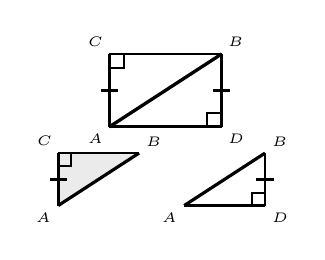
\begin{tikzpicture}[scale=0.50, every node/.style={font=\tiny, text=black}]
      % Book p.165 Ex. #12: C top-left, B top-right, A bottom-left, D bottom-right (cyclic trace C-B-D-A)
      \coordinate (A) at (0, 0); \coordinate (D) at (2.85, 0);
      \coordinate (C) at (0, 1.85); \coordinate (B) at (2.85, 1.85);
      \draw[black, line width=1.05pt] (C)--(B) (A)--(D);
      \draw[black, line width=1.1pt, tk1] (C)--(A);
      \draw[black, line width=1.1pt, tk1] (B)--(D);
      \draw[black, line width=1.2pt] (A)--(B);
      \pic[draw=black, line width=0.75pt, angle radius=1.8mm]{right angle=A--C--B};
      \pic[draw=black, line width=0.75pt, angle radius=1.8mm]{right angle=B--D--A};
      \node[above left=-1pt] at (C) {$C$}; \node[above right=-1pt] at (B) {$B$};
      \node[below left=-1pt] at (A) {$A$}; \node[below right=-1pt] at (D) {$D$};
      % Exploded ∆ACB (left) and ∆BDA (right) centered under [0..2.85]
      \begin{scope}[shift={(-1.30, -2.00)}, scale=0.72]
        \coordinate (a1) at (0,0); \coordinate (c1) at (0,1.85); \coordinate (b1) at (2.85,1.85);
        \fill[panelgray] (a1)--(c1)--(b1)--cycle;
        \draw[black, line width=1.0pt, tk1] (a1)--(c1);
        \draw[black, line width=0.95pt] (c1)--(b1);
        \draw[black, line width=1.15pt] (a1)--(b1);
        \pic[draw=black, line width=0.7pt, angle radius=1.6mm]{right angle=a1--c1--b1};
        \node[below left=-1pt] at (a1) {$A$}; \node[above left=-1pt] at (c1) {$C$}; \node[above right=-1pt] at (b1) {$B$};
      \end{scope}
      \begin{scope}[shift={(1.90, -2.00)}, scale=0.72]
        \coordinate (a2) at (0,0); \coordinate (d2) at (2.85,0); \coordinate (b2) at (2.85,1.85);
        \fill[white] (a2)--(d2)--(b2)--cycle;
        \draw[black, line width=1.0pt, tk1] (b2)--(d2);
        \draw[black, line width=0.95pt] (a2)--(d2);
        \draw[black, line width=1.15pt] (a2)--(b2);
        \pic[draw=black, line width=0.7pt, angle radius=1.6mm]{right angle=b2--d2--a2};
        \node[below left=-1pt] at (a2) {$A$}; \node[below right=-1pt] at (d2) {$D$}; \node[above right=-1pt] at (b2) {$B$};
      \end{scope}
    \end{tikzpicture}
  \end{minipage}

  \vspace{3.5pt}
  \begin{tcolorbox}[
    enhanced, sharp corners, colback=panelgray, colframe=black,
    boxrule=0.75pt, boxsep=1pt, top=3pt, bottom=3pt, left=4pt, right=4pt
  ]
    \fontsize{6.9pt}{9.9pt}\selectfont
    \textbf{ផ្ទៀងខ្លួនឯង (\en{Warrant \cnum{1}--\cnum{5}})៖}
    \chkbox\ គូស $90^\circ$ ($BD\perp AC, CE\perp AB$ និង $\ang{C}=\ang{D}=90^\circ$) + ព្រួញអ៊ីប៉ូតេនុសរួម ($BC$, $AB$)!\\
    \chkbox\ សរសេរលក្ខខណ្ឌ \textbf{អ.ជ (\en{HL})} ទាំង ៣ បន្ទាត់ឱ្យច្បាស់ (មុំ $90^\circ$, អ៊ីប៉ូតេនុសរួម, ជ្រុងកែងស្មើ)!\\
    \chkbox\ ដាក់លេខ \cnum{1}--\cnum{5} គ្រប់បន្ទាត់ និងទាញមុំឆ្លាស់ក្នុង $\ang{CBA}=\ang{DAB} \Rightarrow BC \parallel AD$ (លំ.១២)។
  \end{tcolorbox}
\end{tcolorbox}%
}

\noindent
\hwslipFourHL{ប័ណ្ណទី ១}\hfill\hwslipFourHL{ប័ណ្ណទី ២}

\vspace{7pt}
\noindent\scissors\ \dotfill\ \textbf{កាត់តាមស្នាមចុចចែកជា ៤ ប័ណ្ណ (\en{Cut Along Dashed Lines})} \dotfill\ \scissors
\vspace{7pt}

\noindent
\hwslipFourHL{ប័ណ្ណទី ៣}\hfill\hwslipFourHL{ប័ណ្ណទី ៤}

\end{document}
